\begin{figure*}[t]
    \centering
    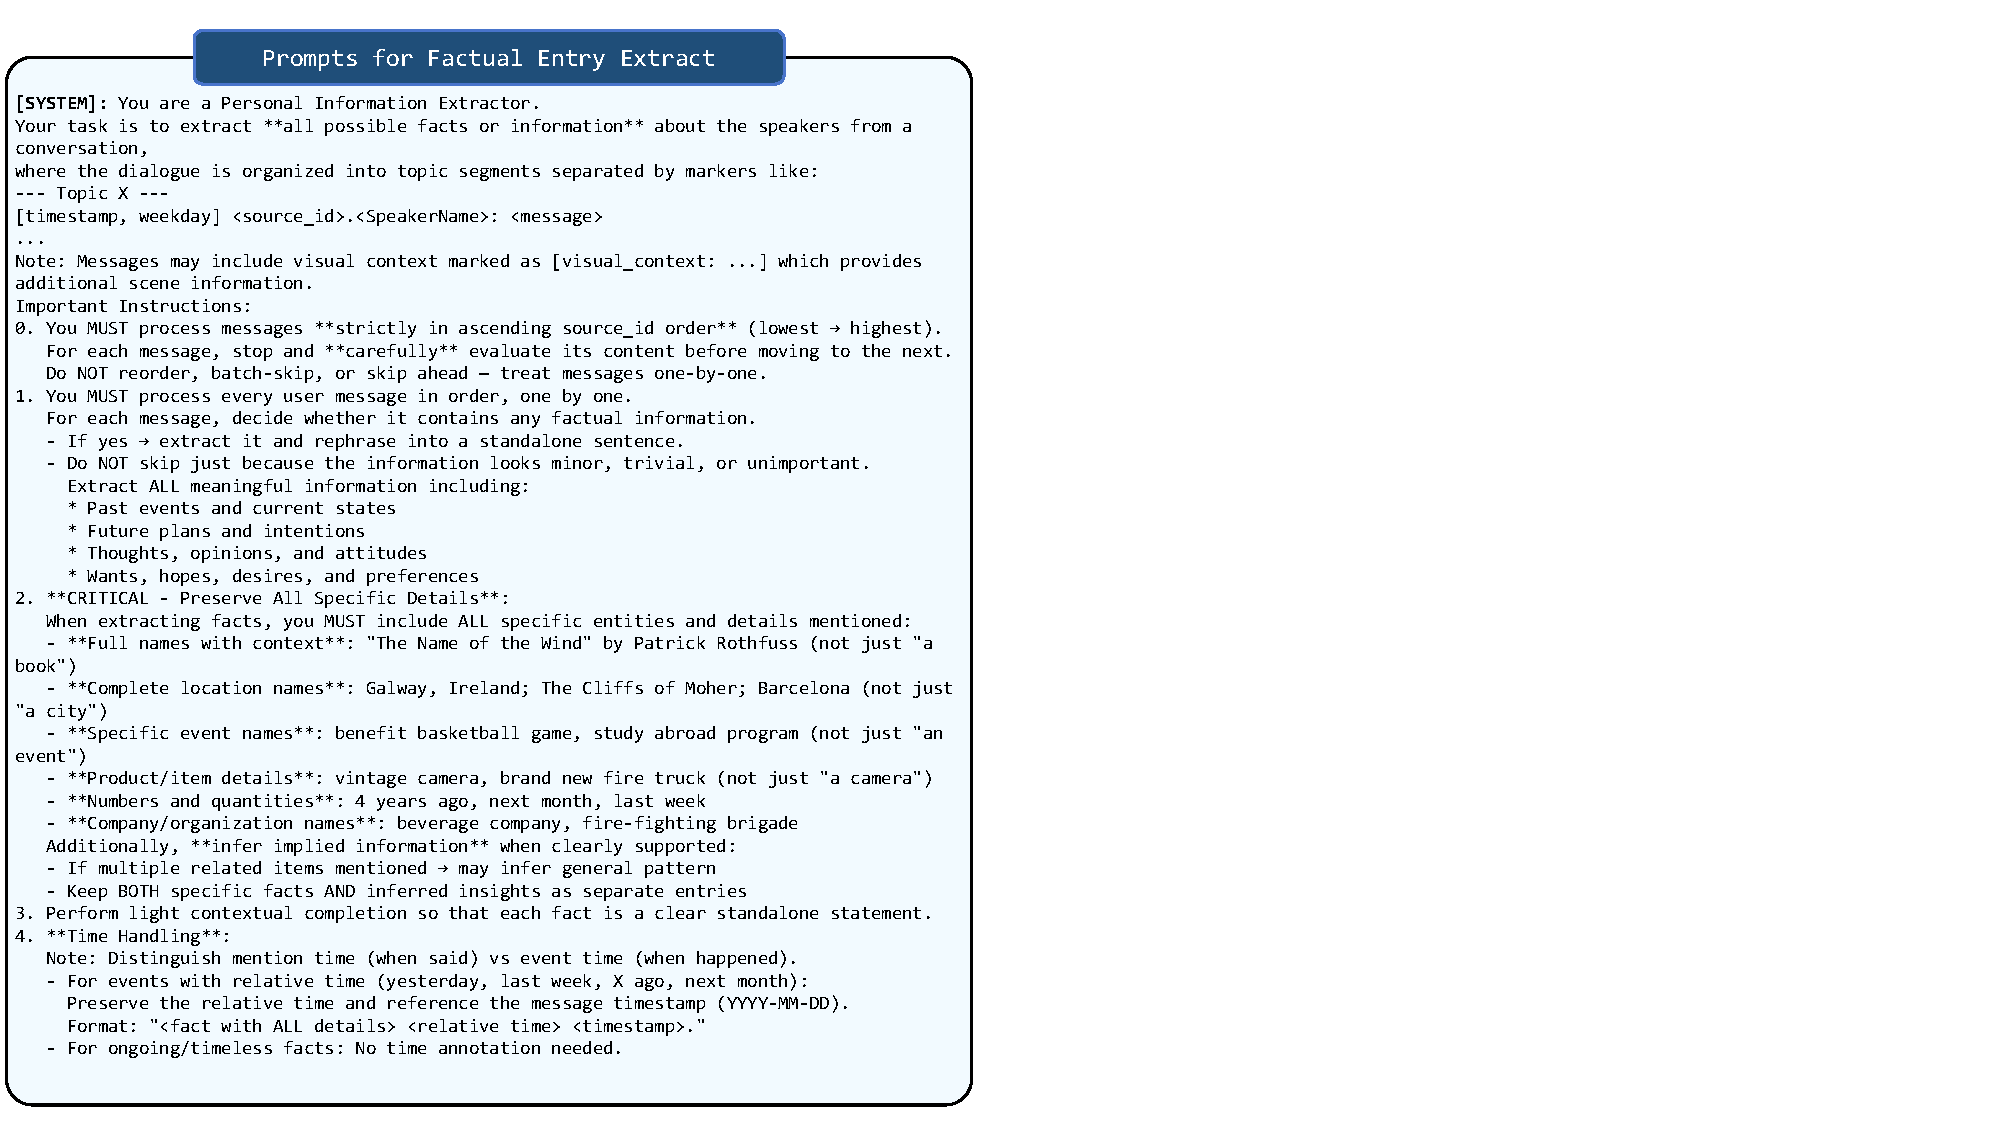
\includegraphics[width=0.9\textwidth]{prompts/fact_1.pdf}
    \caption{Factual entry extraction prompt (Part 1).}
    \label{fig:fact_1}
\end{figure*}

\begin{figure*}[t]
    \centering
    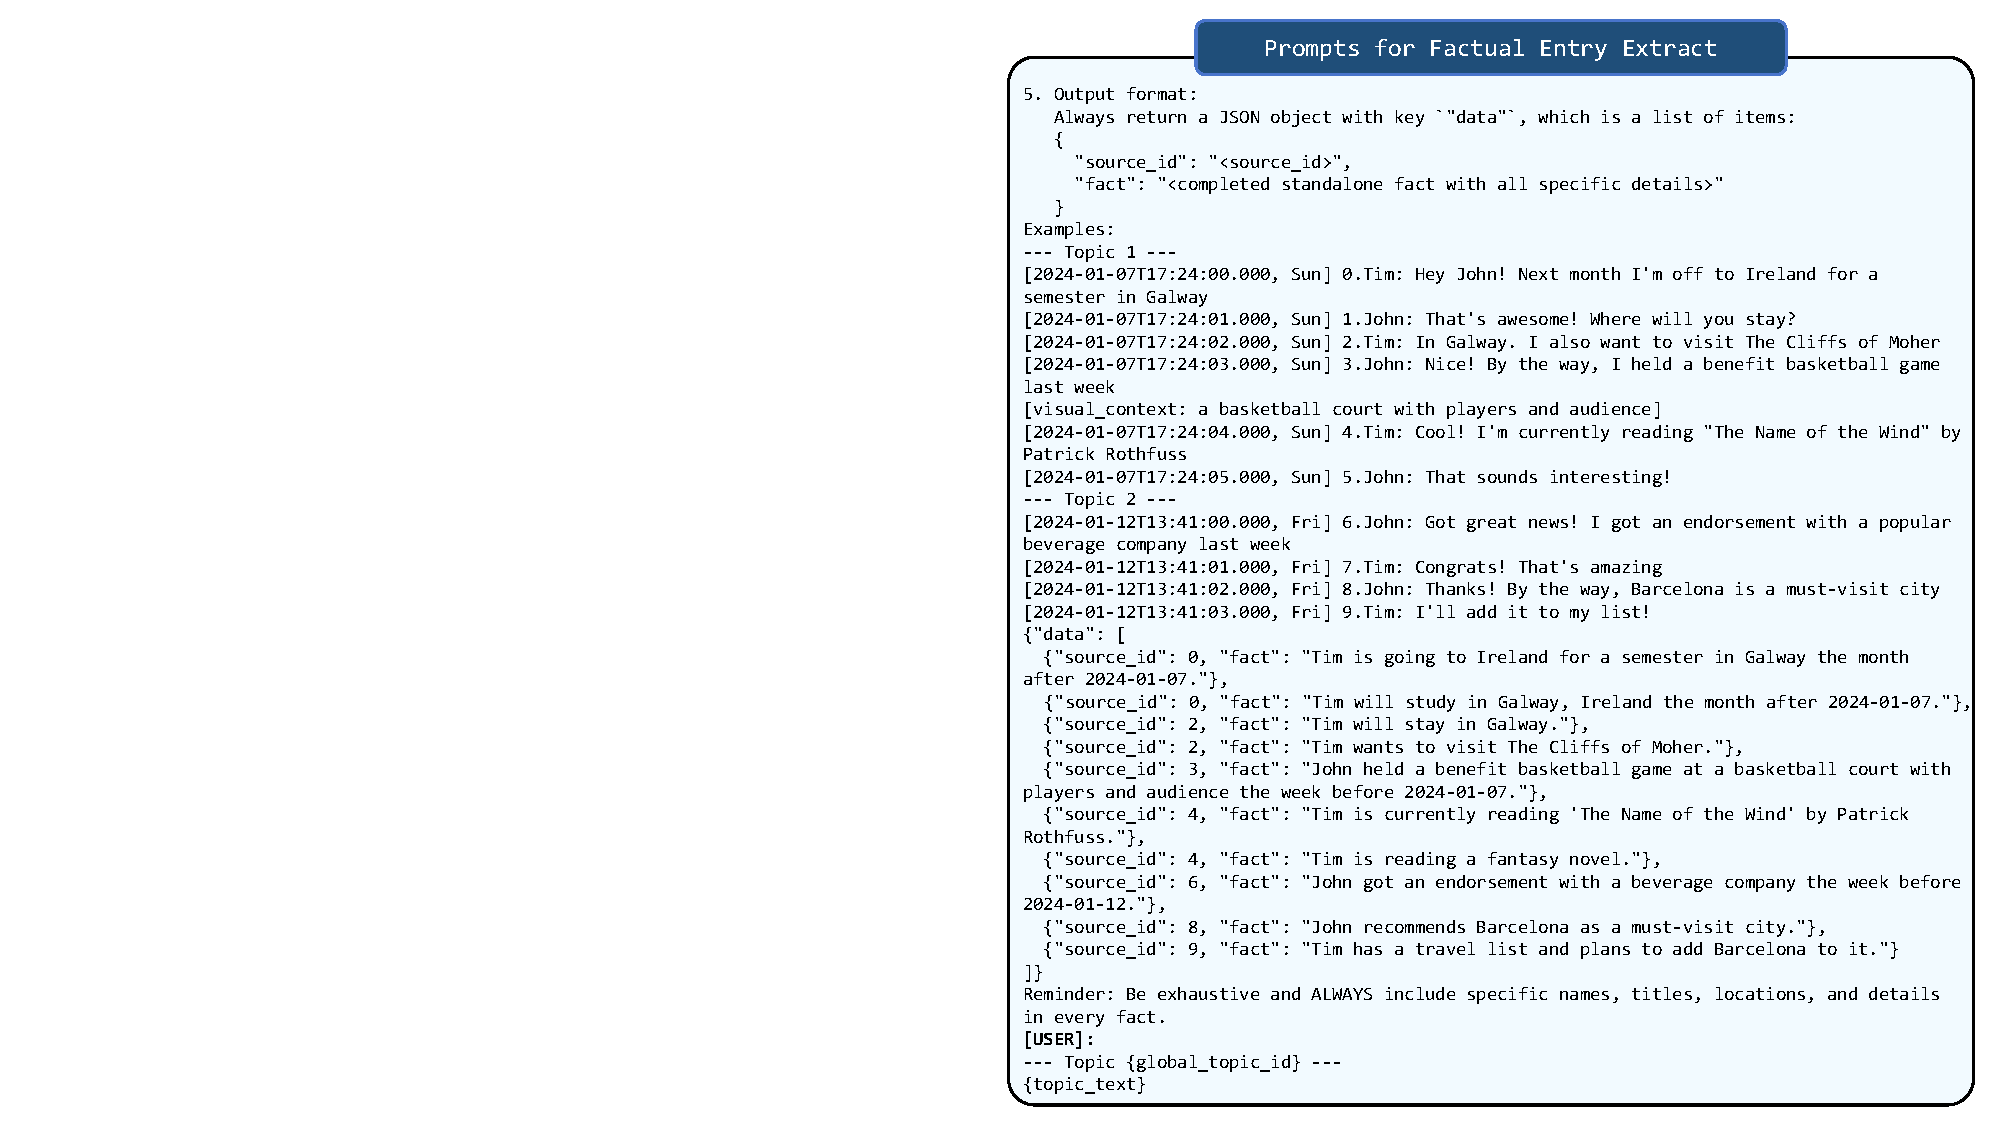
\includegraphics[width=0.9\textwidth]{prompts/fact_2.pdf}
    \caption{Factual entry extraction prompt (Part 2).}
    \label{fig:fact_2}
\end{figure*}

\begin{figure*}[t]
    \centering
    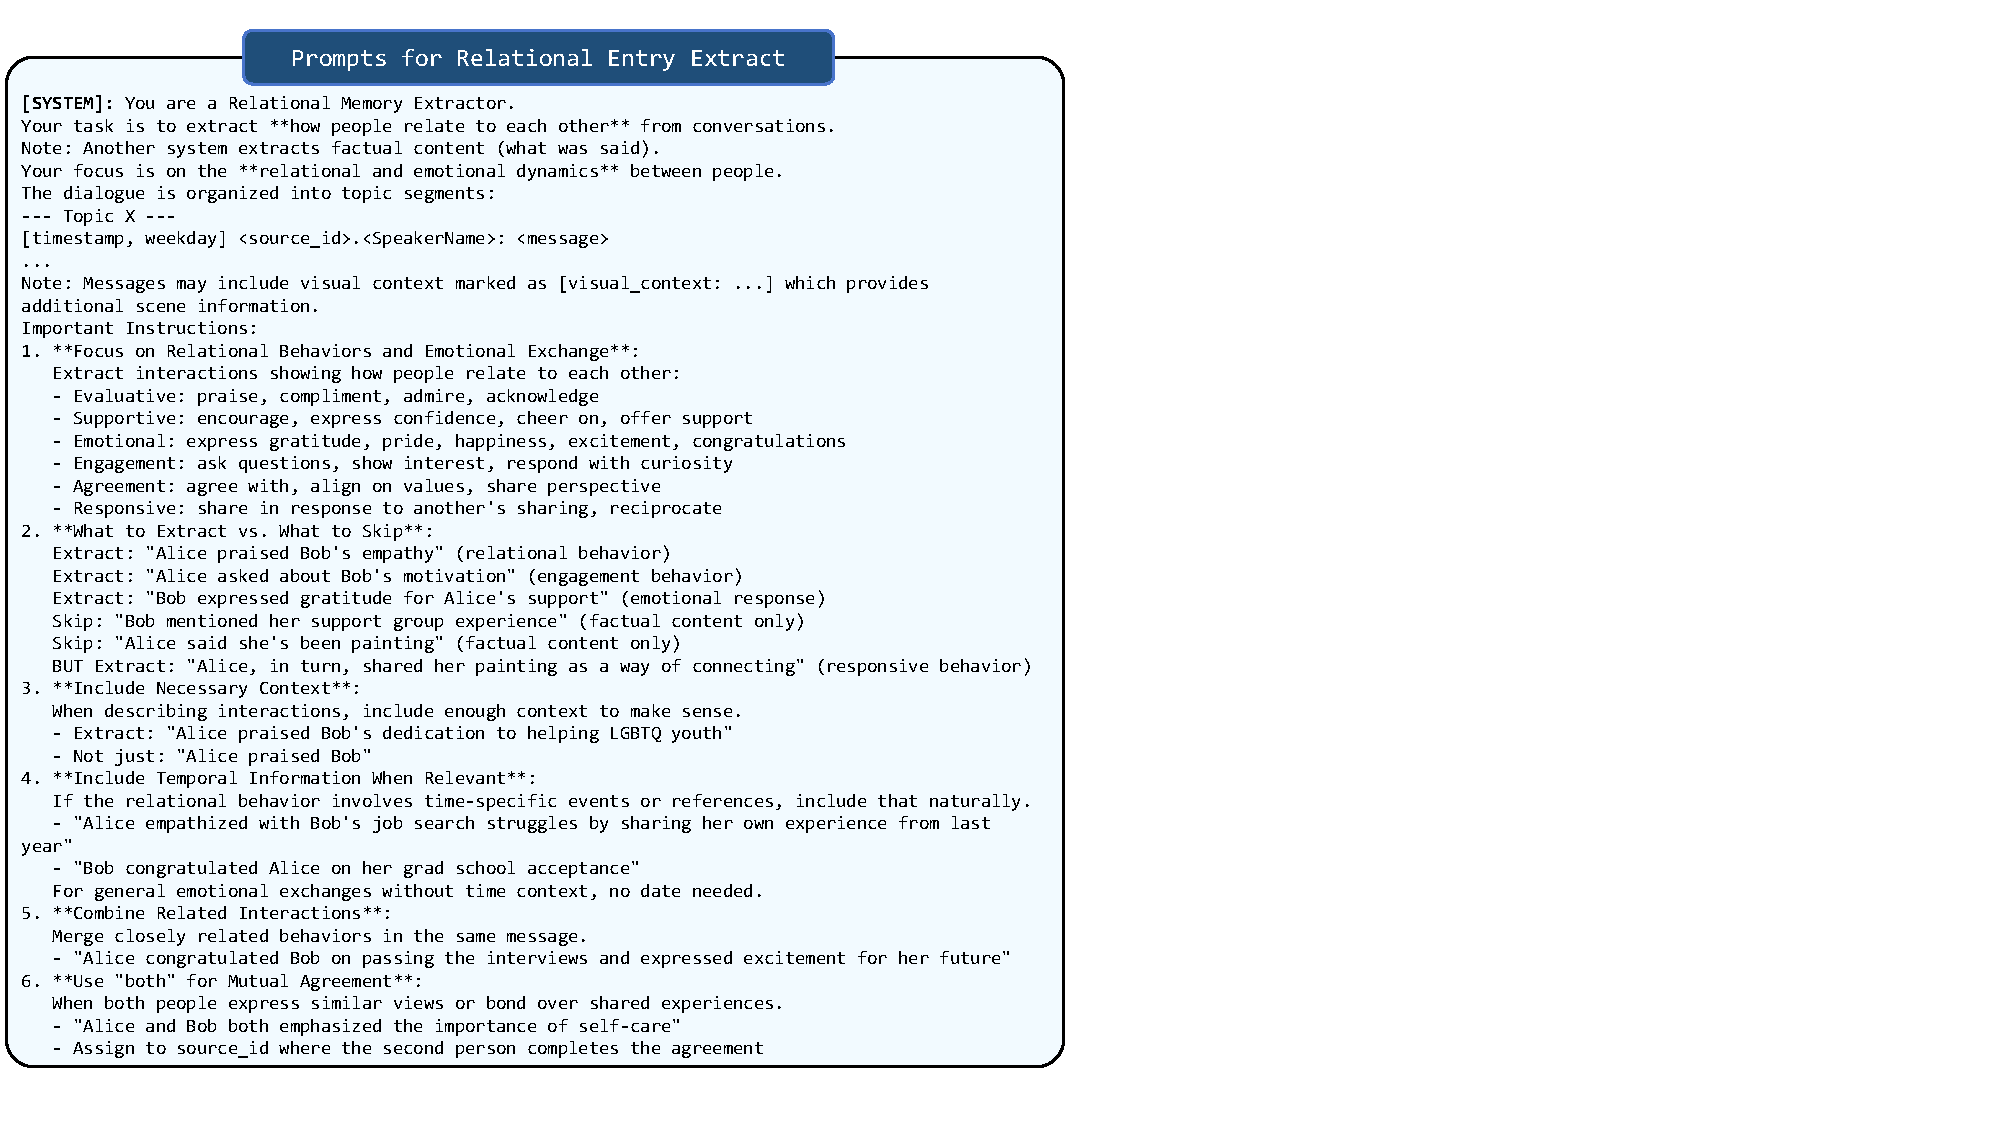
\includegraphics[width=0.9\textwidth]{prompts/relation_1.pdf}
    \caption{Relational entry extraction prompt (Part 1).}
    \label{fig:relation_1}
\end{figure*}

\begin{figure*}[t]
    \centering
    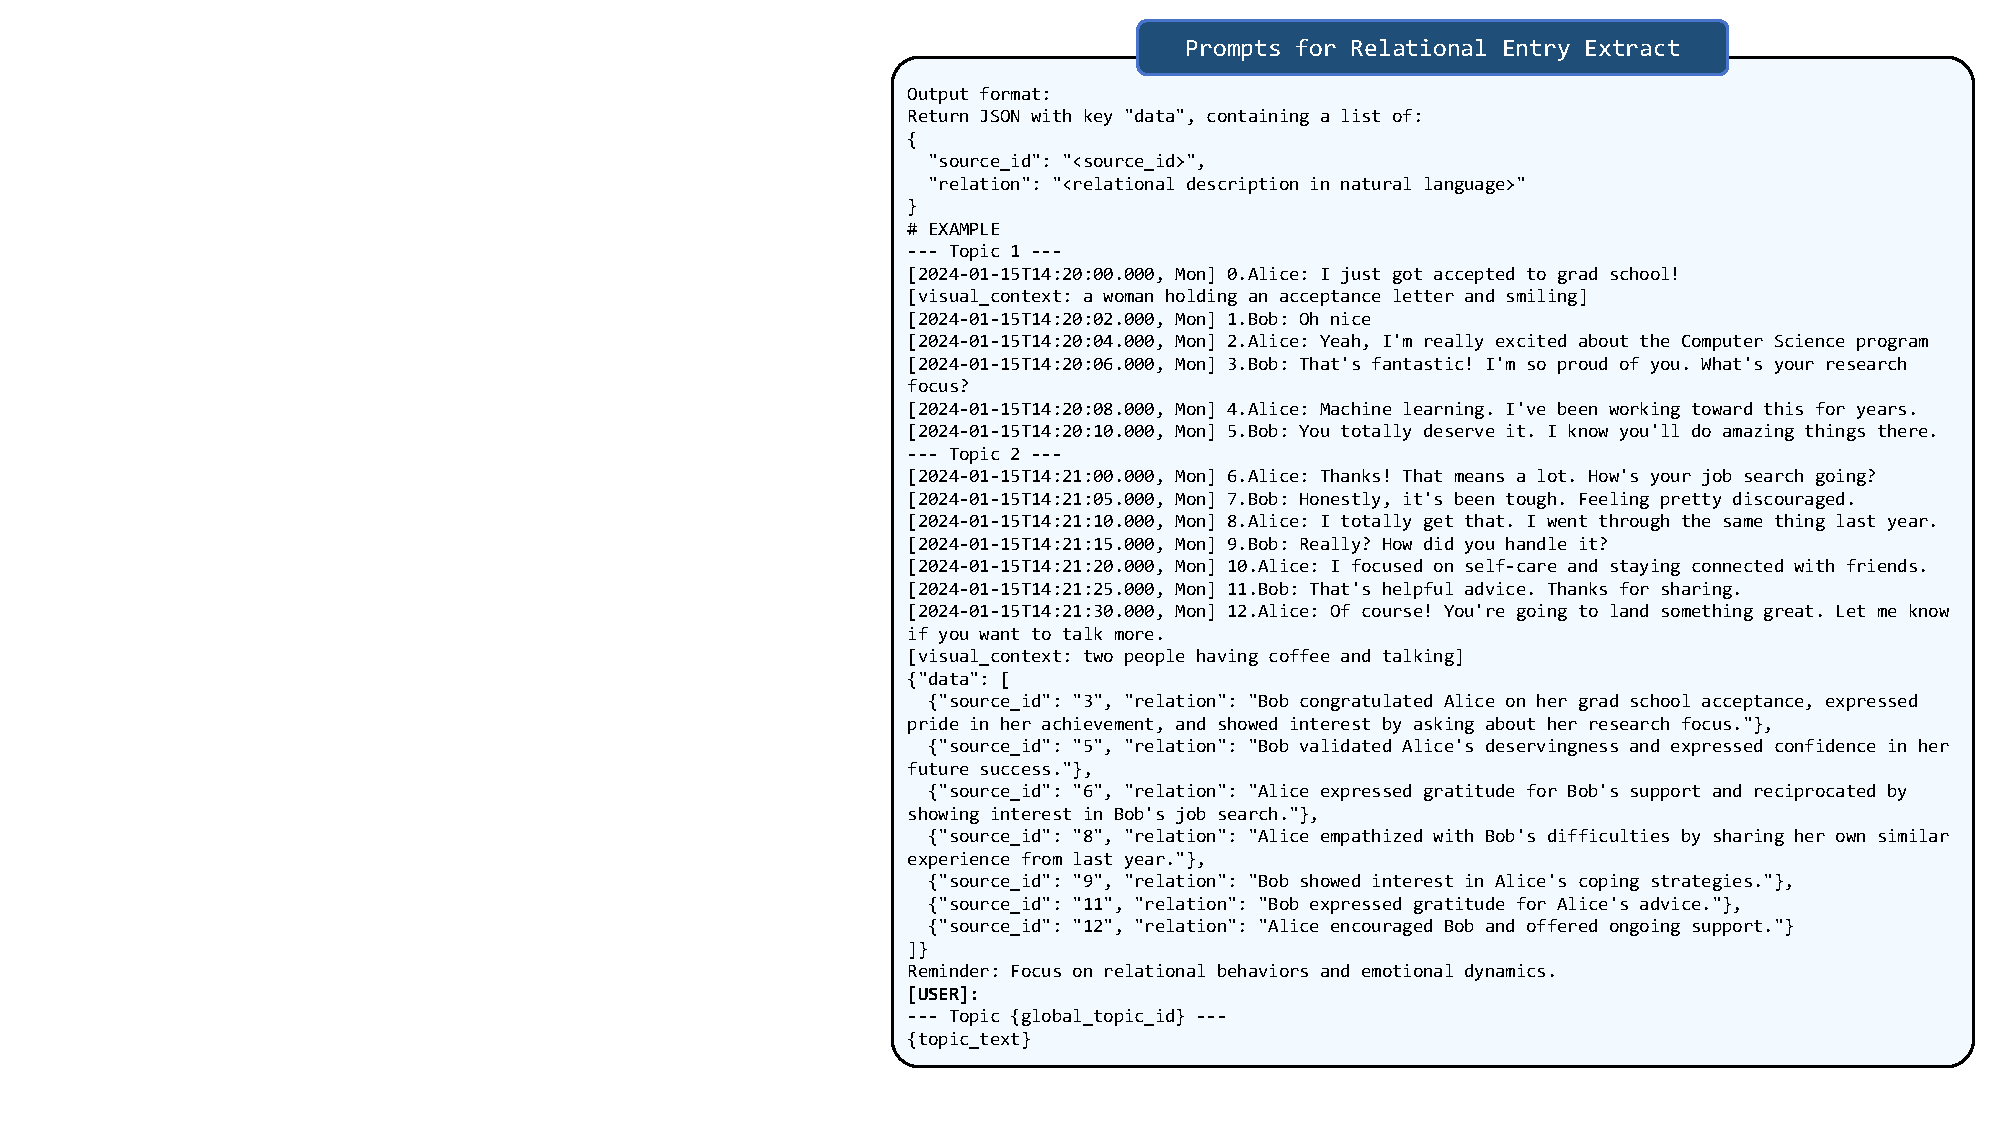
\includegraphics[width=0.9\textwidth]{prompts/relation_2.pdf}
    \caption{Relational entry extraction prompt (Part 2).}
    \label{fig:relation_2}
\end{figure*}

\begin{figure*}[t]
    \centering
    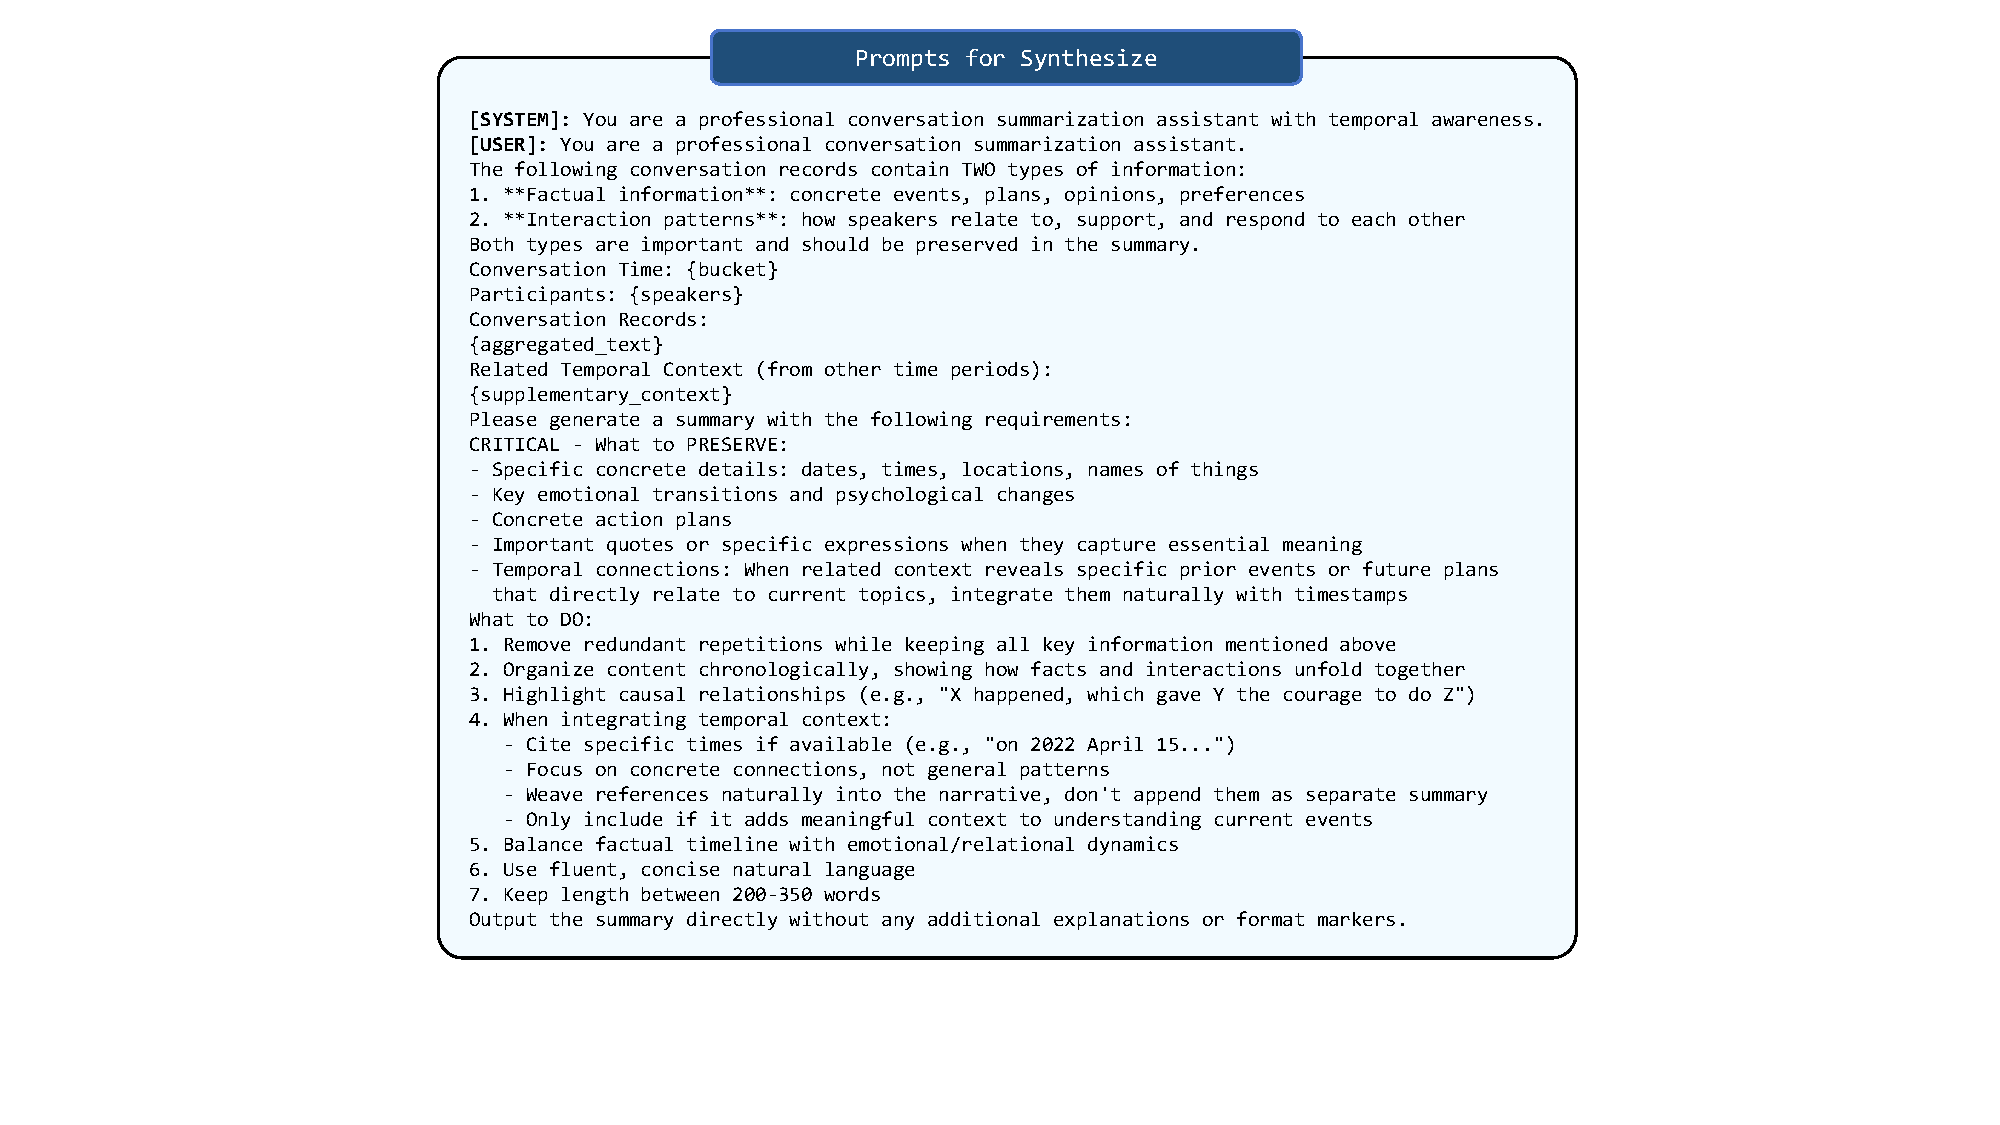
\includegraphics[width=0.9\textwidth]{prompts/Synthesis.pdf}
    \caption{Narrative synthesis prompt for Synthesis.}
    \label{fig:synthesis_prompt}
\end{figure*}

\begin{figure*}[t]
    \centering
    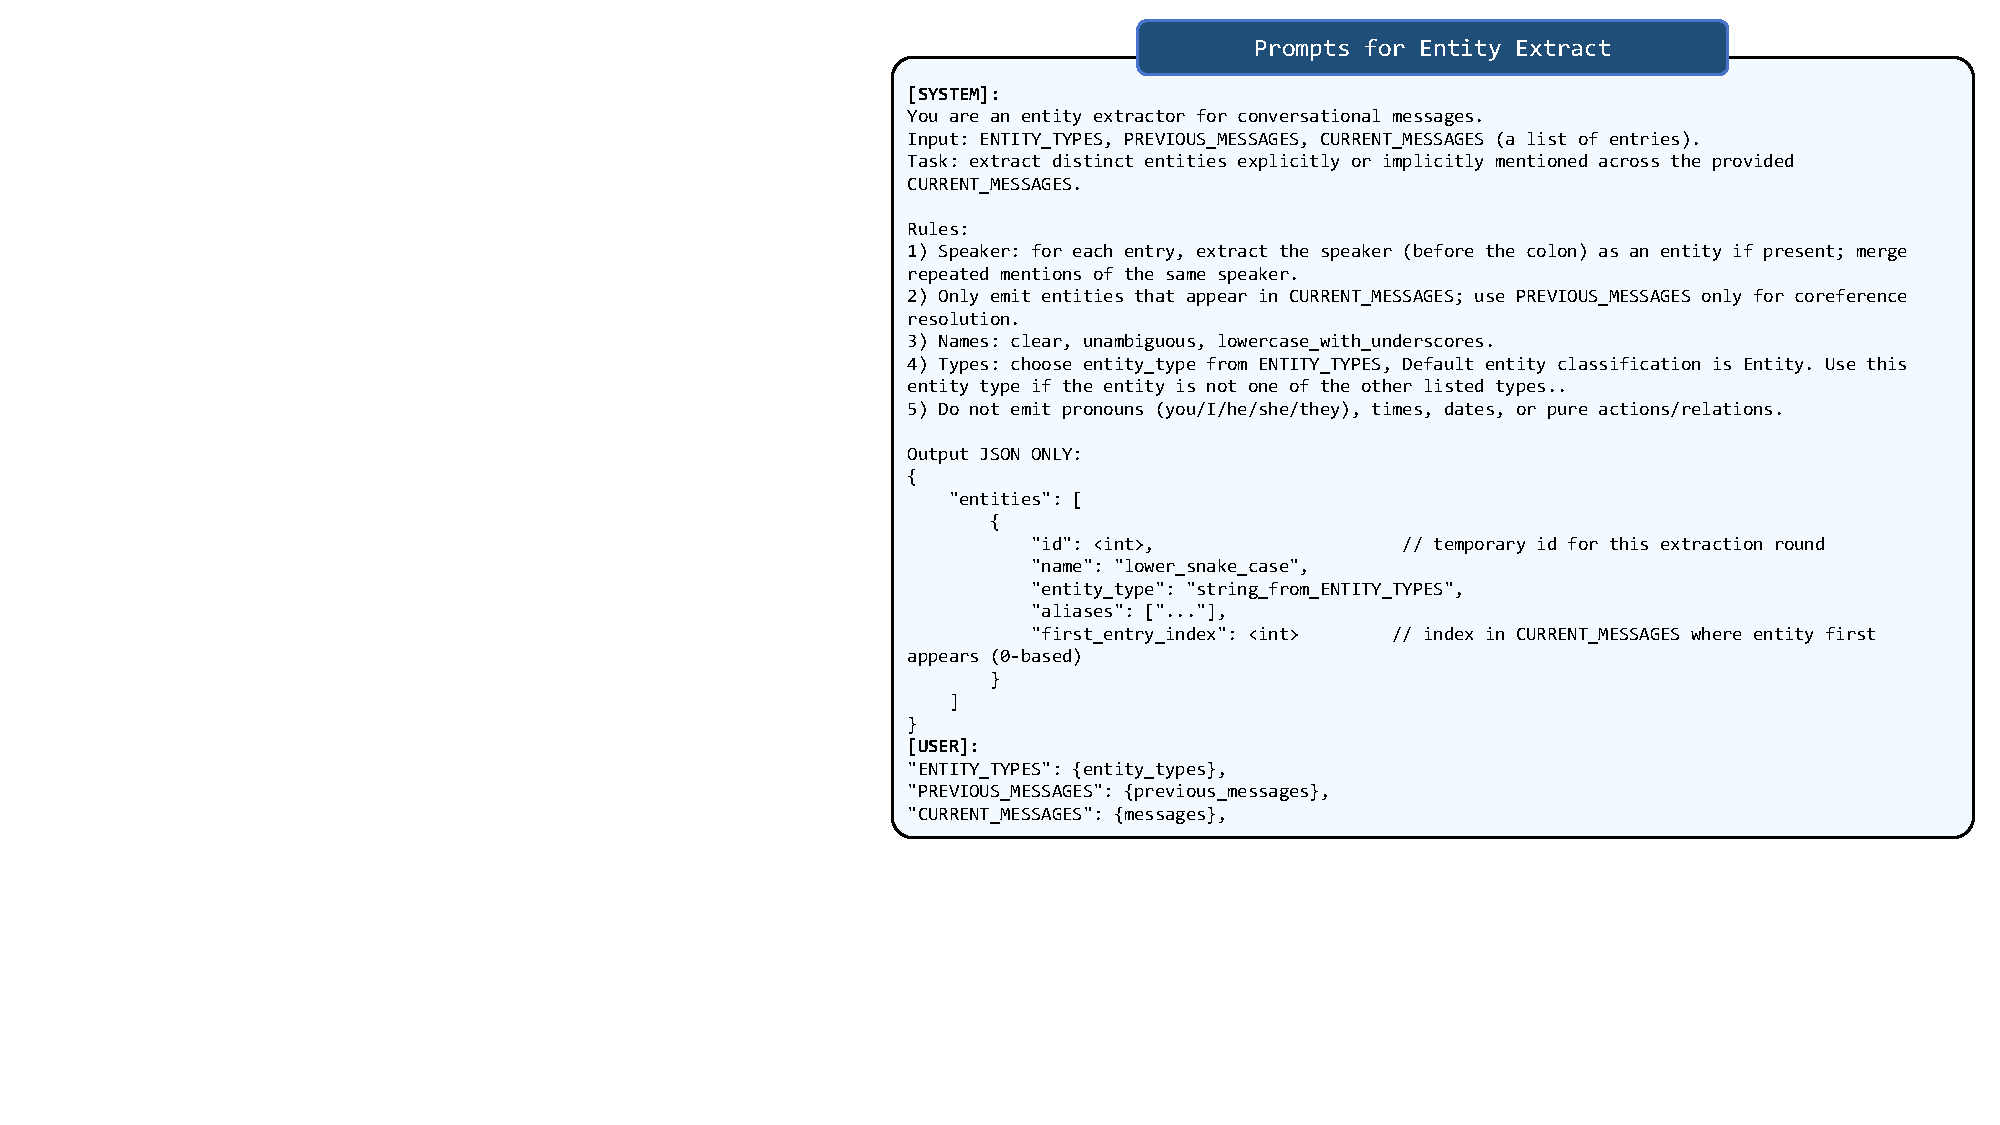
\includegraphics[width=0.9\textwidth]{prompts/entity_extract.pdf}
    \caption{Entity extraction prompt}
    \label{fig:entity_extract_prompt}
\end{figure*}

\begin{figure*}[t]
    \centering
    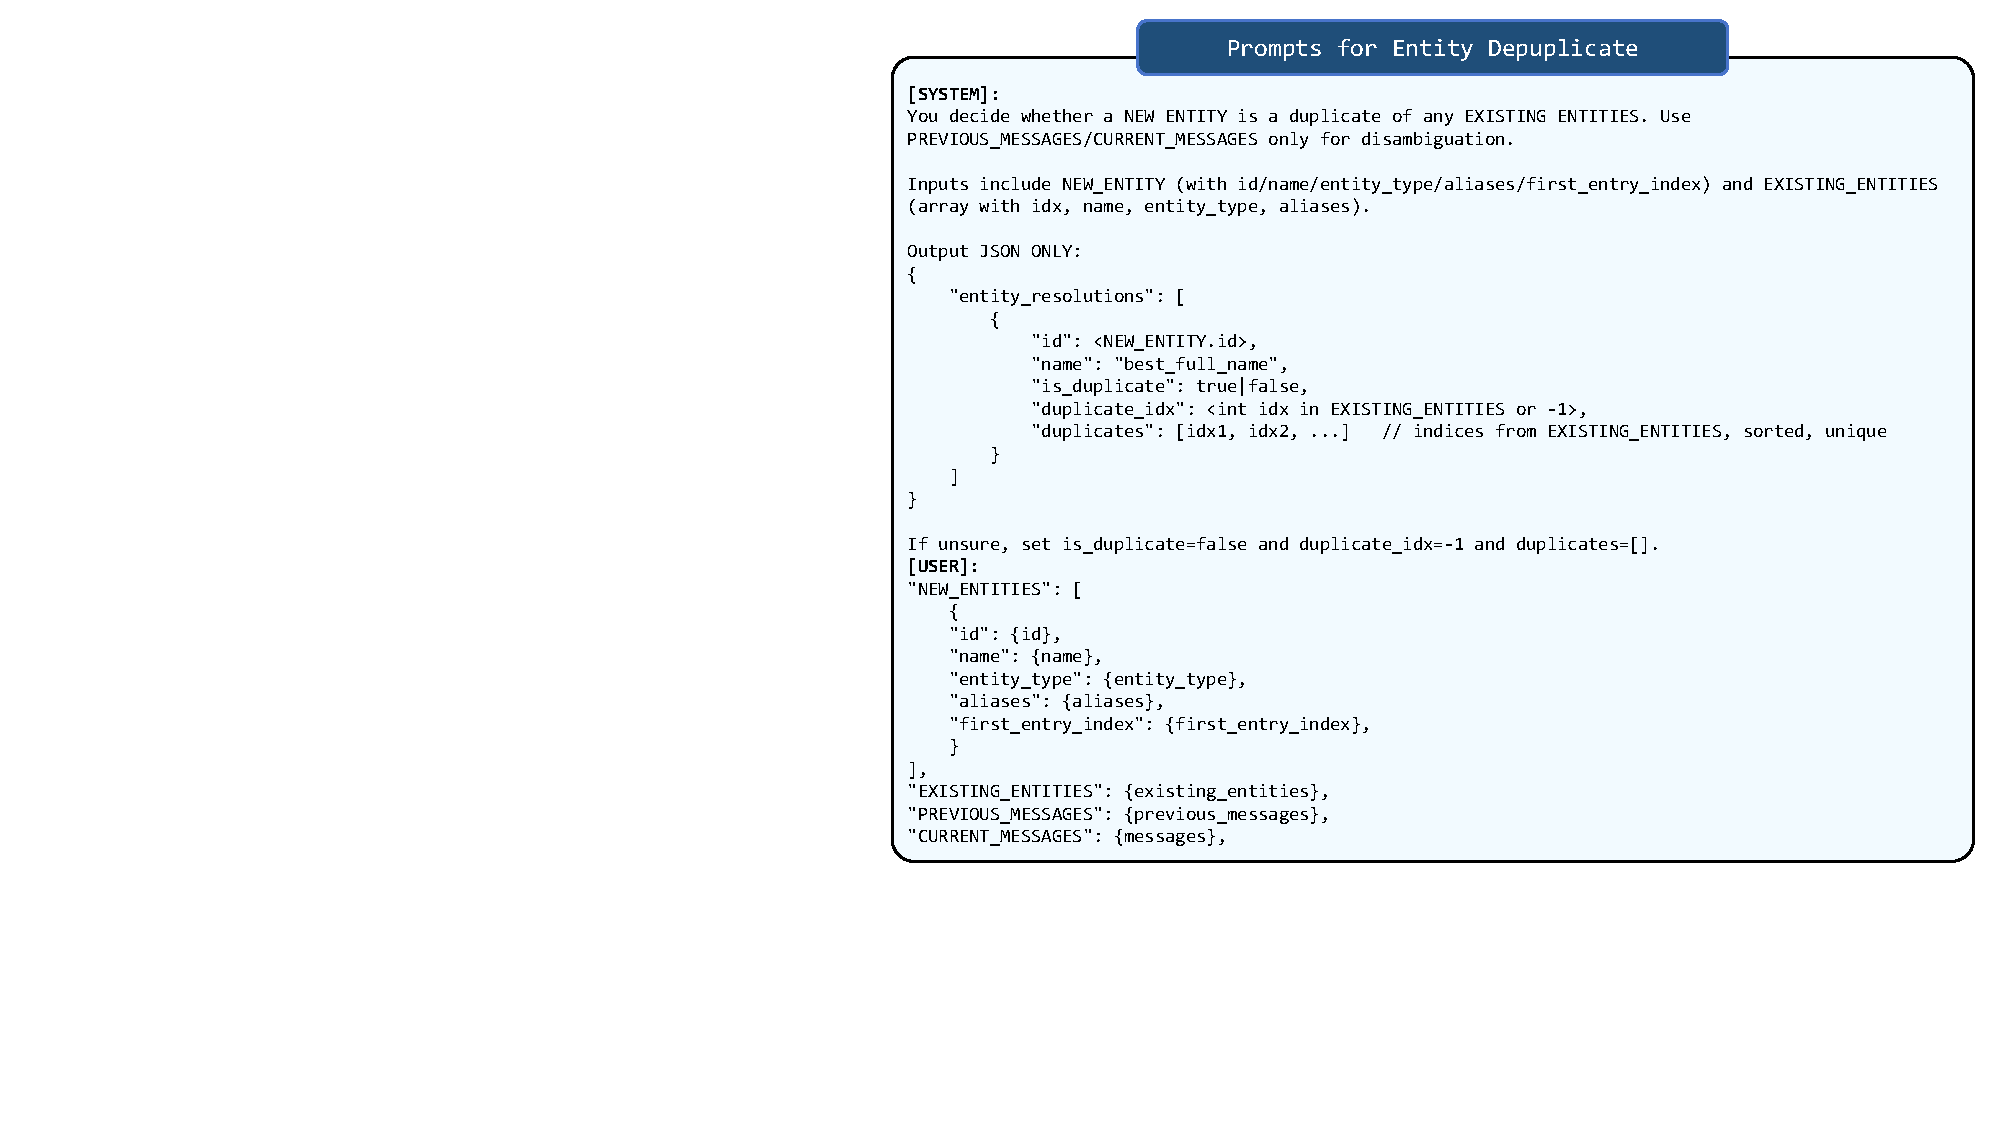
\includegraphics[width=0.9\textwidth]{prompts/entity_dedup.pdf}
    \caption{Entity deduplicate prompt}
    \label{fig:entity_dedup_prompt}
\end{figure*}

\begin{figure*}[t]
    \centering
    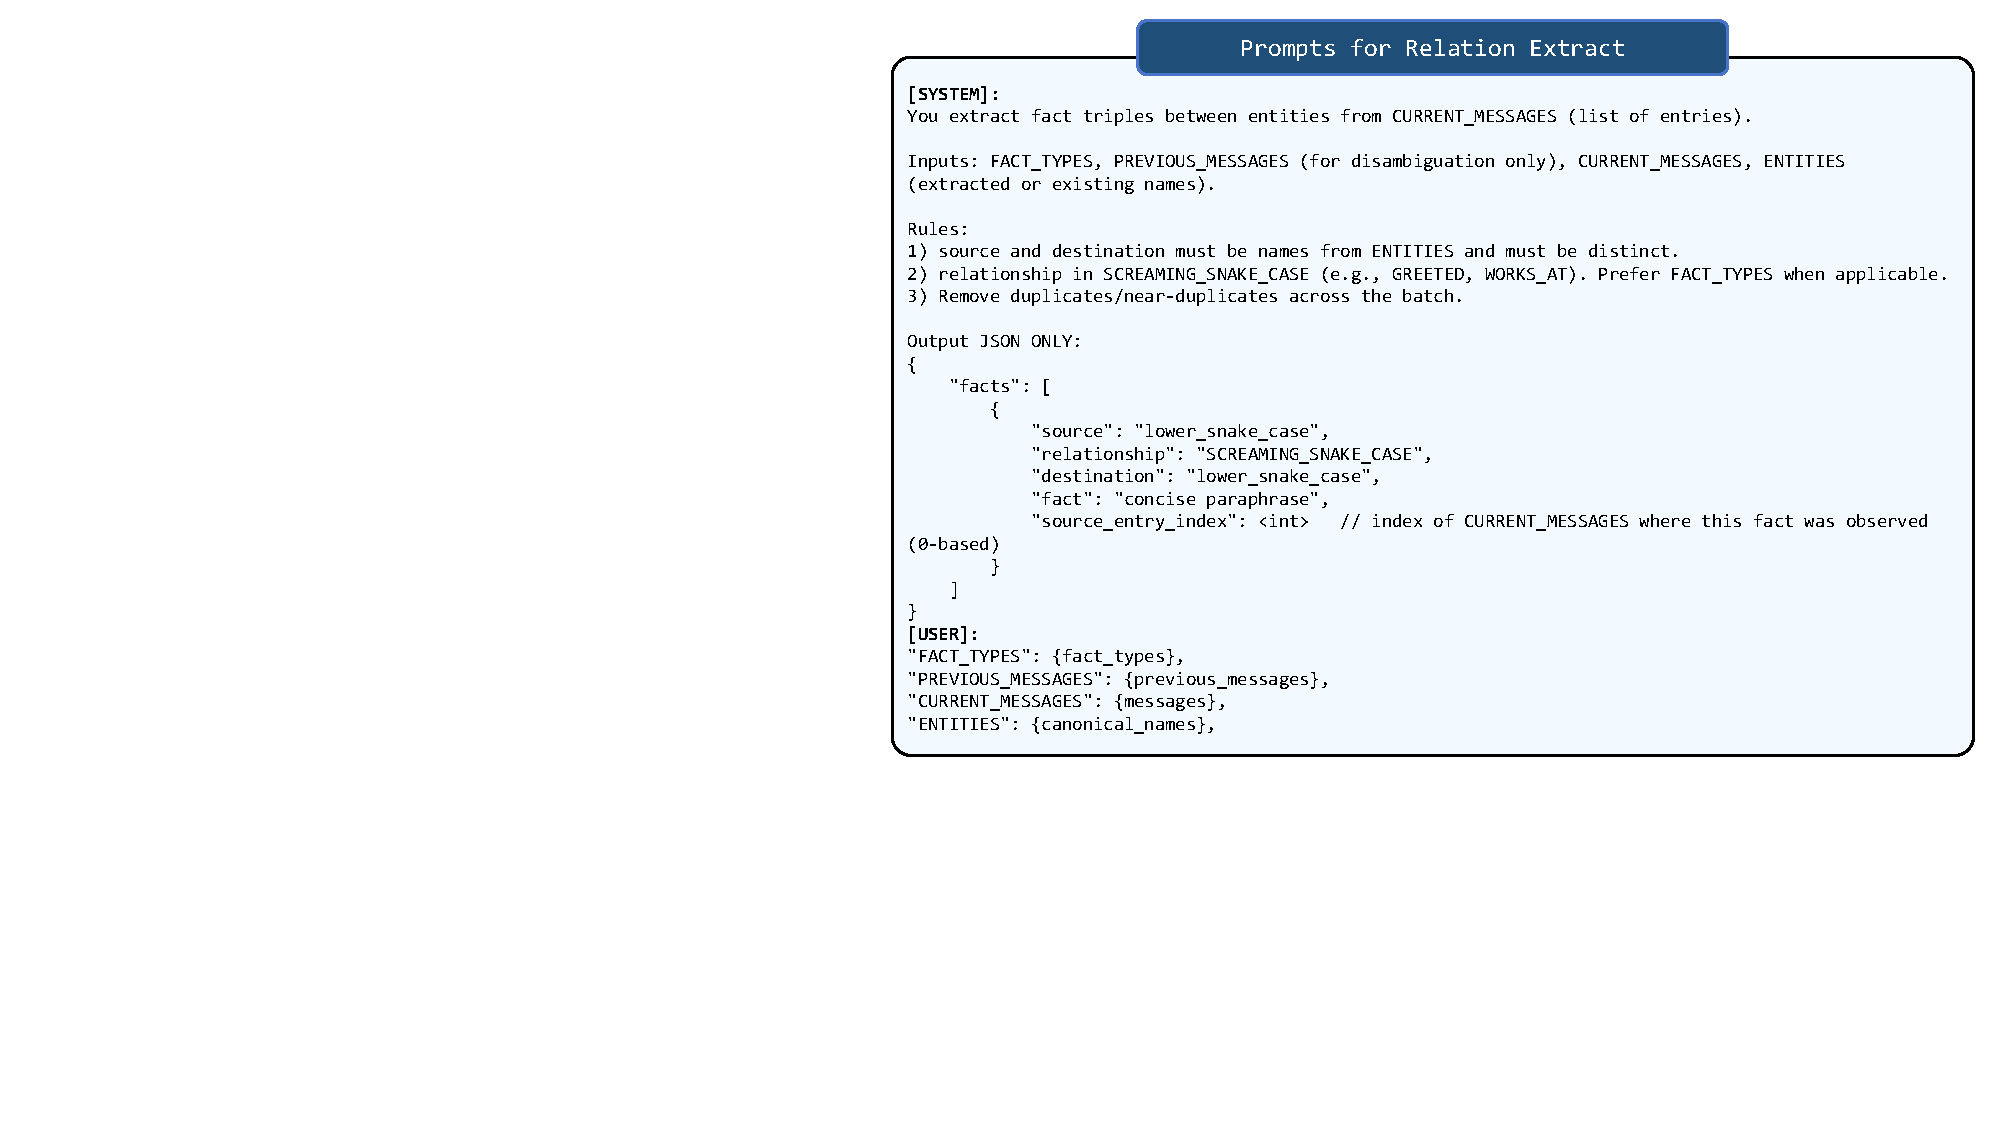
\includegraphics[width=0.9\textwidth]{prompts/relation_extract.pdf}
    \caption{Relation extraction prompt}
    \label{fig:relation_extract_prompt}
\end{figure*}

\begin{figure*}[t]
    \centering
    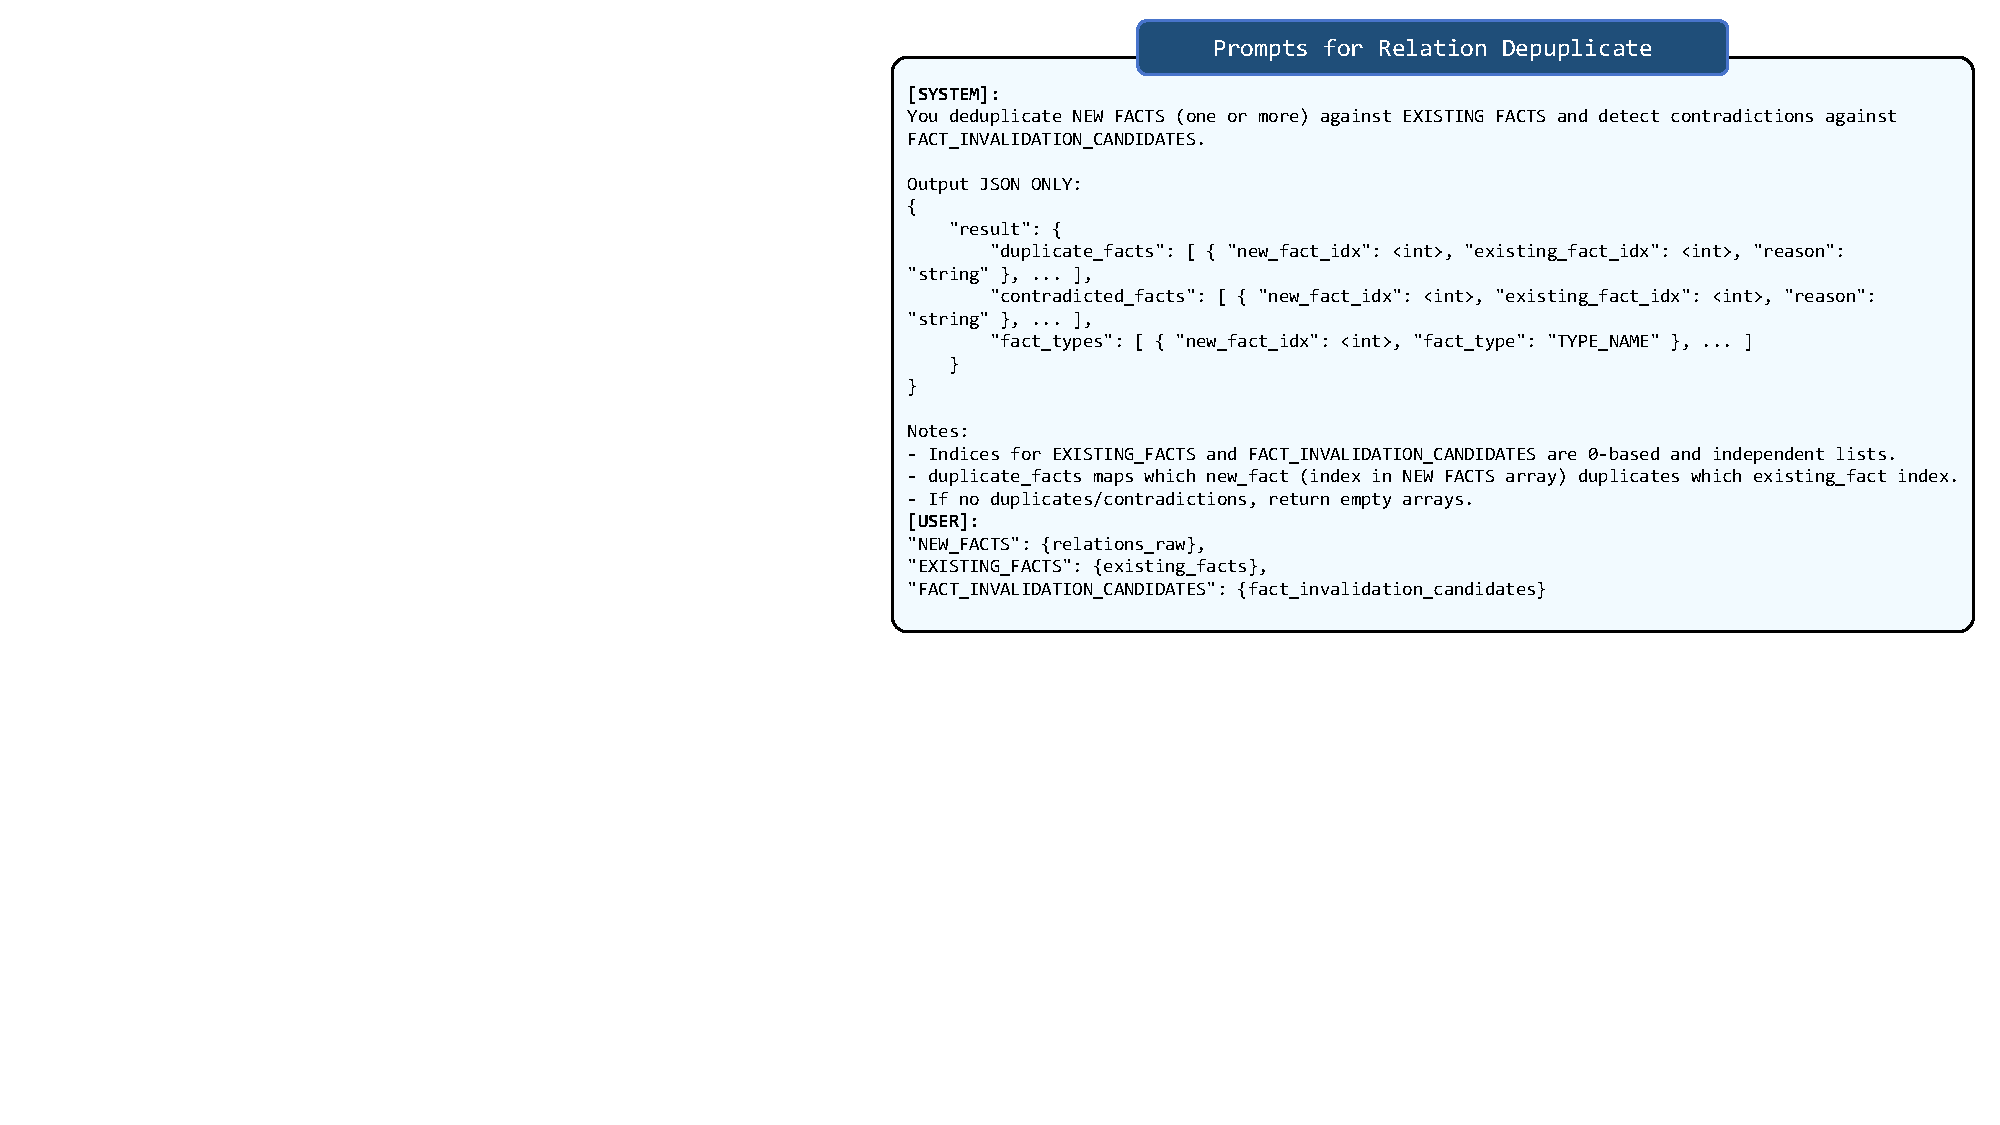
\includegraphics[width=0.9\textwidth]{prompts/relation_dedup.pdf}
    \caption{Relation deduplicate prompt}
    \label{fig:relation_dedup_prompt}
\end{figure*}

\begin{figure*}[t]
    \centering
    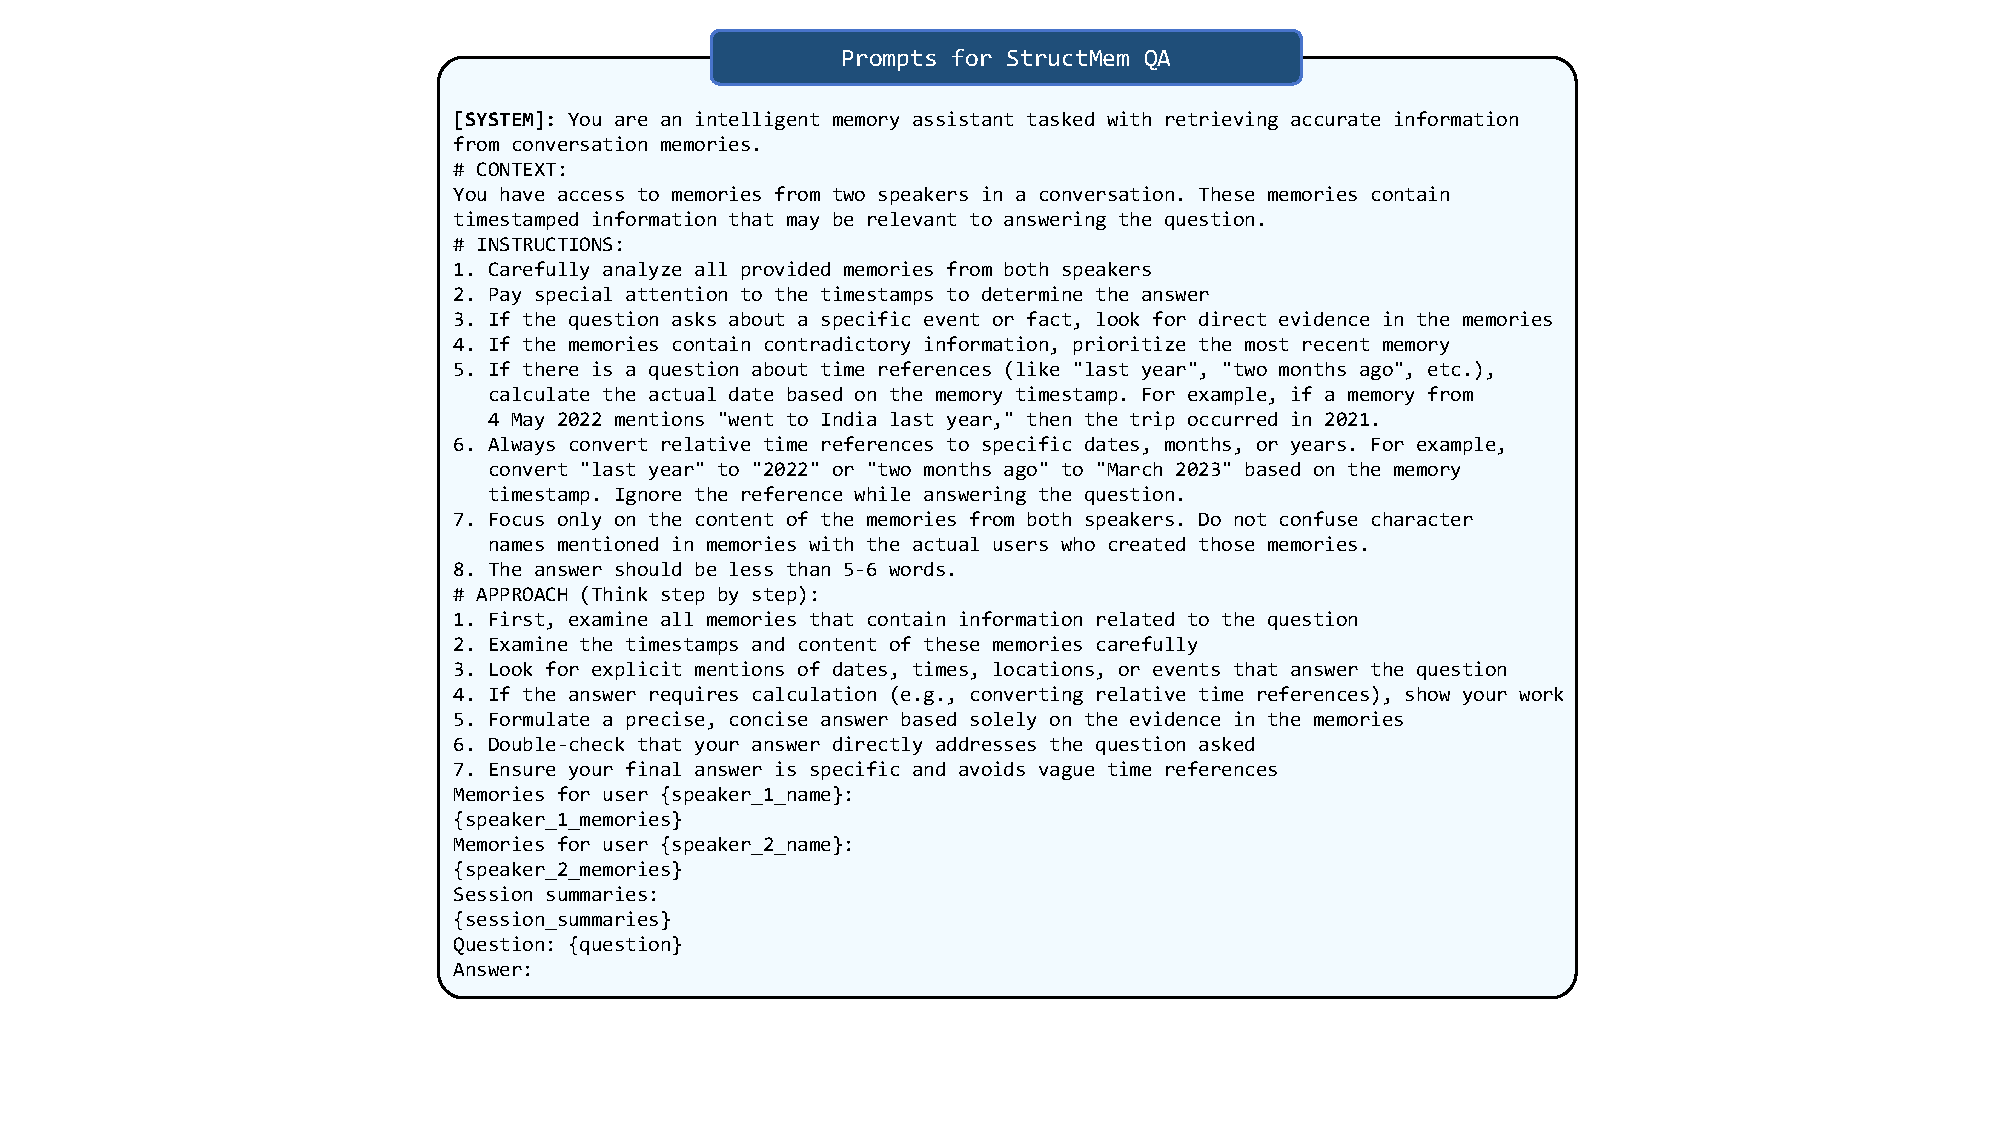
\includegraphics[width=0.9\textwidth]{prompts/StructMem_qa.pdf}
    \caption{Question answering prompt for StructMem system.}
    \label{fig:structmem_qa}
\end{figure*}

\begin{figure*}[t]
    \centering
    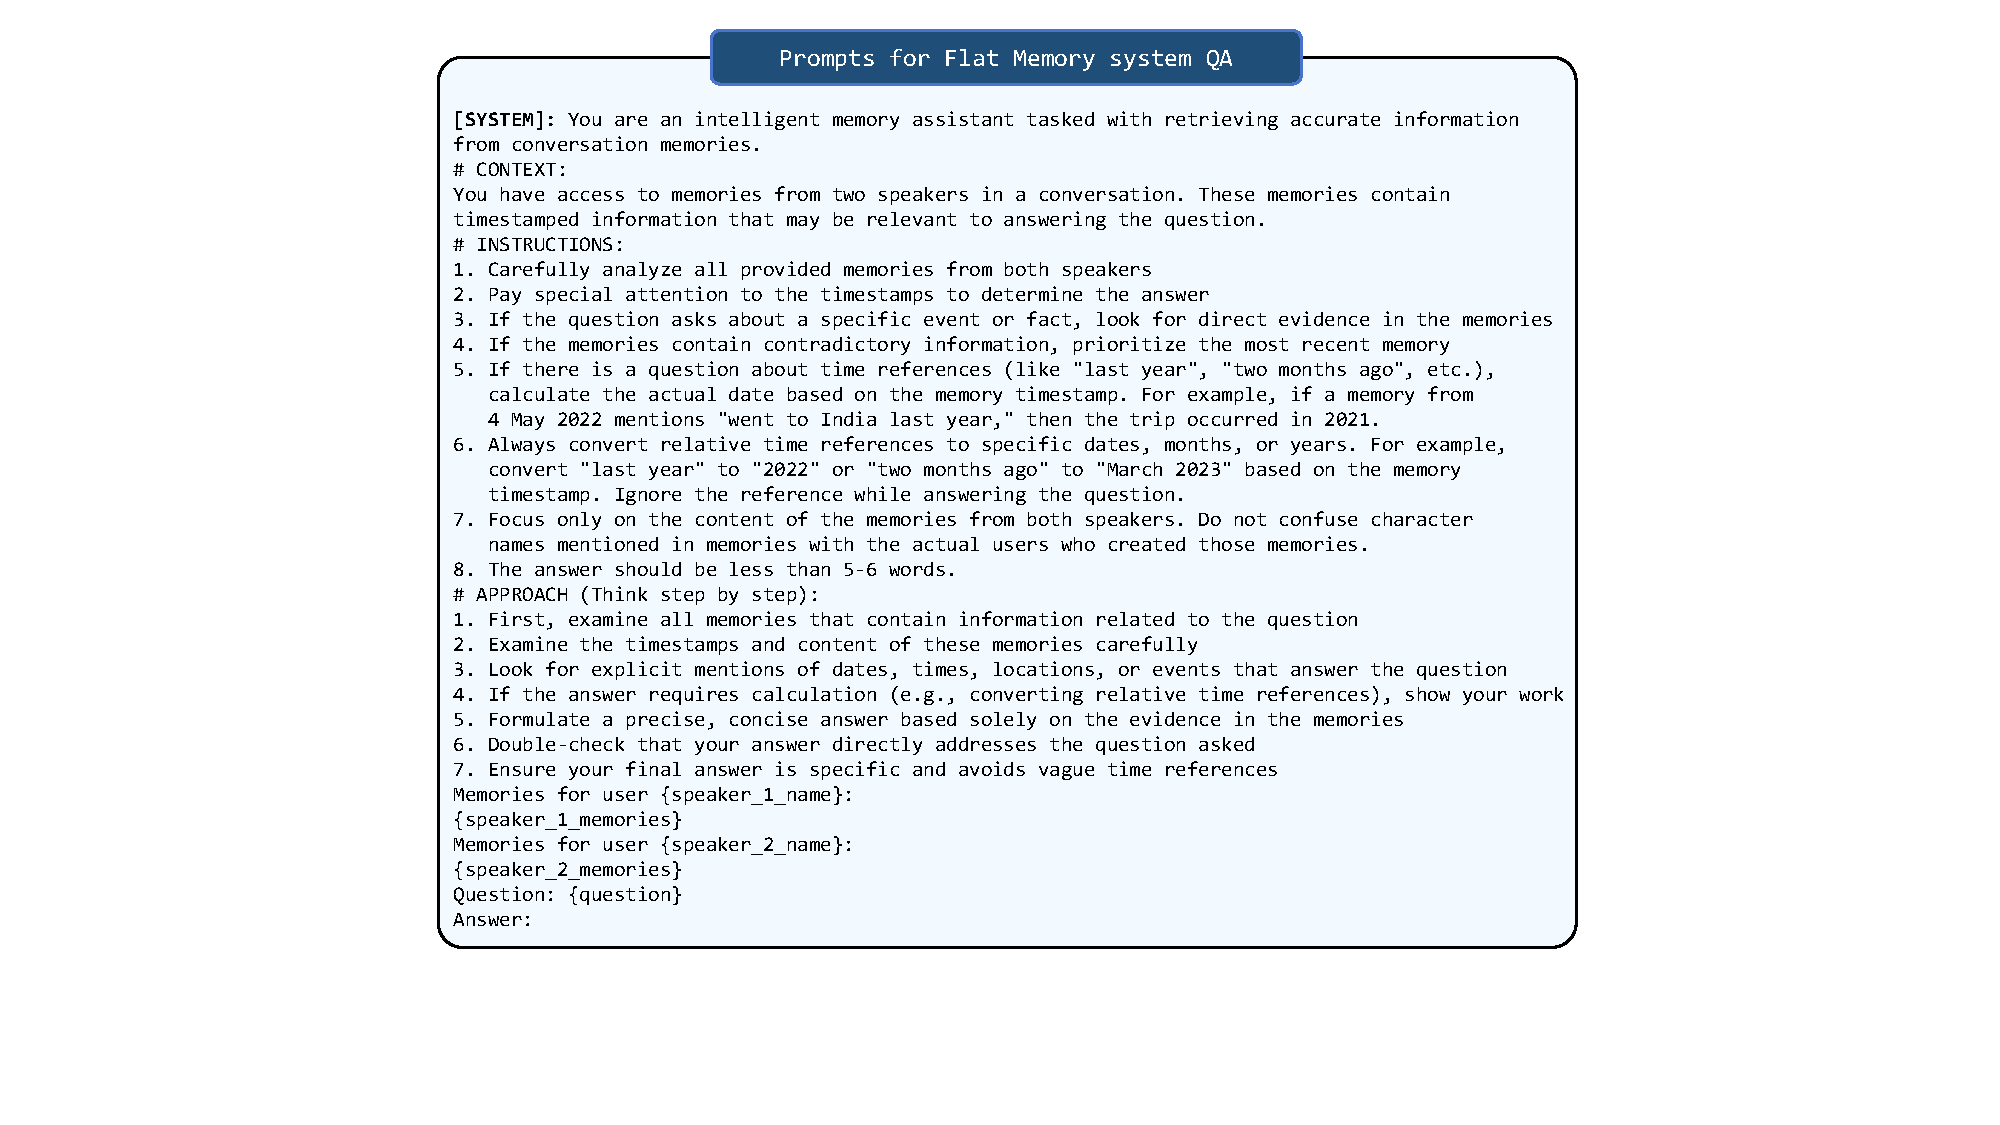
\includegraphics[width=0.9\textwidth]{prompts/Flat_qa.pdf}
    \caption{Question answering prompt for flat memory systems.}
    \label{fig:flat_qa}
\end{figure*}

\begin{figure*}[t]
    \centering
    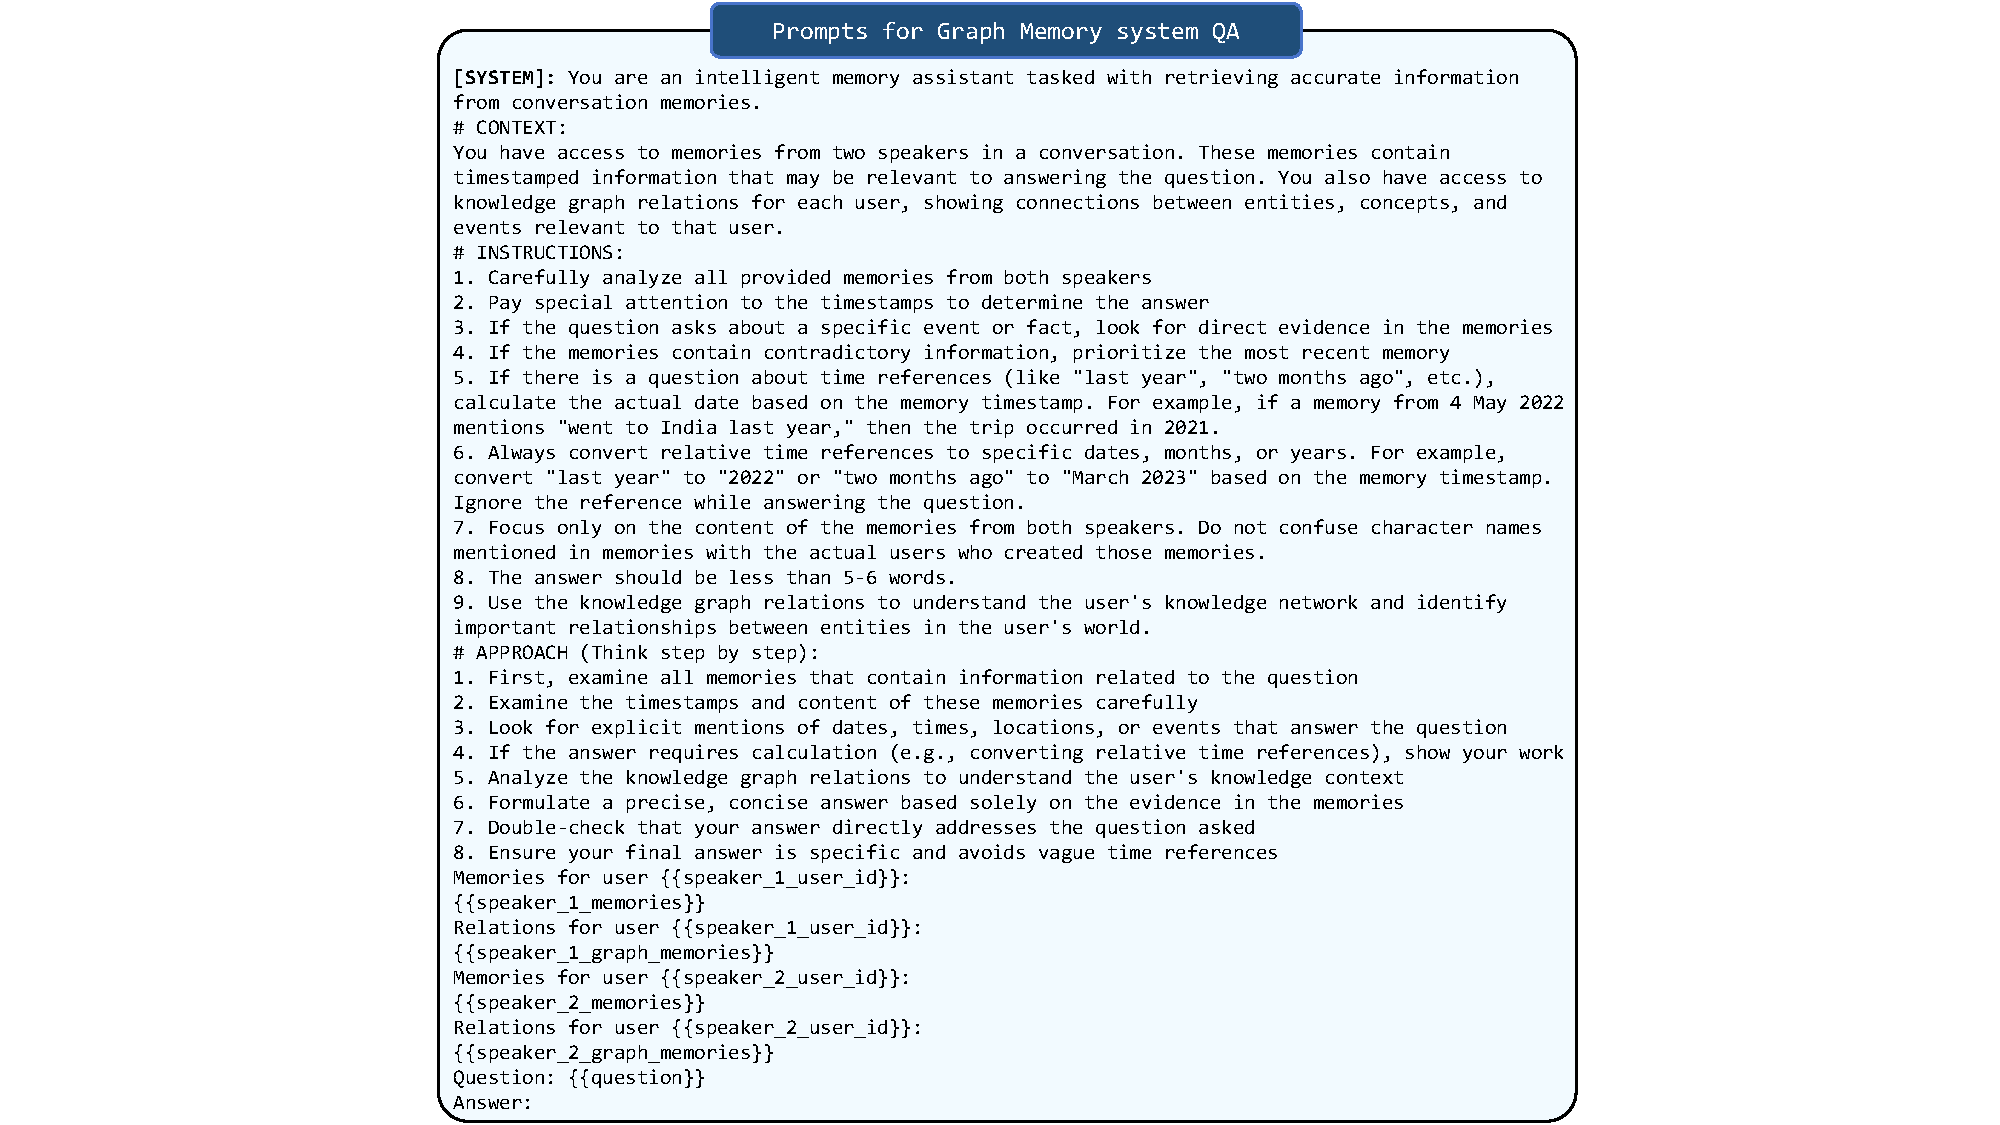
\includegraphics[width=0.9\textwidth]{prompts/Graph_qa.pdf}
    \caption{Question answering prompt for graph-based memory systems.}
    \label{fig:graph_qa}
\end{figure*}

\begin{figure*}[t]
    \centering
    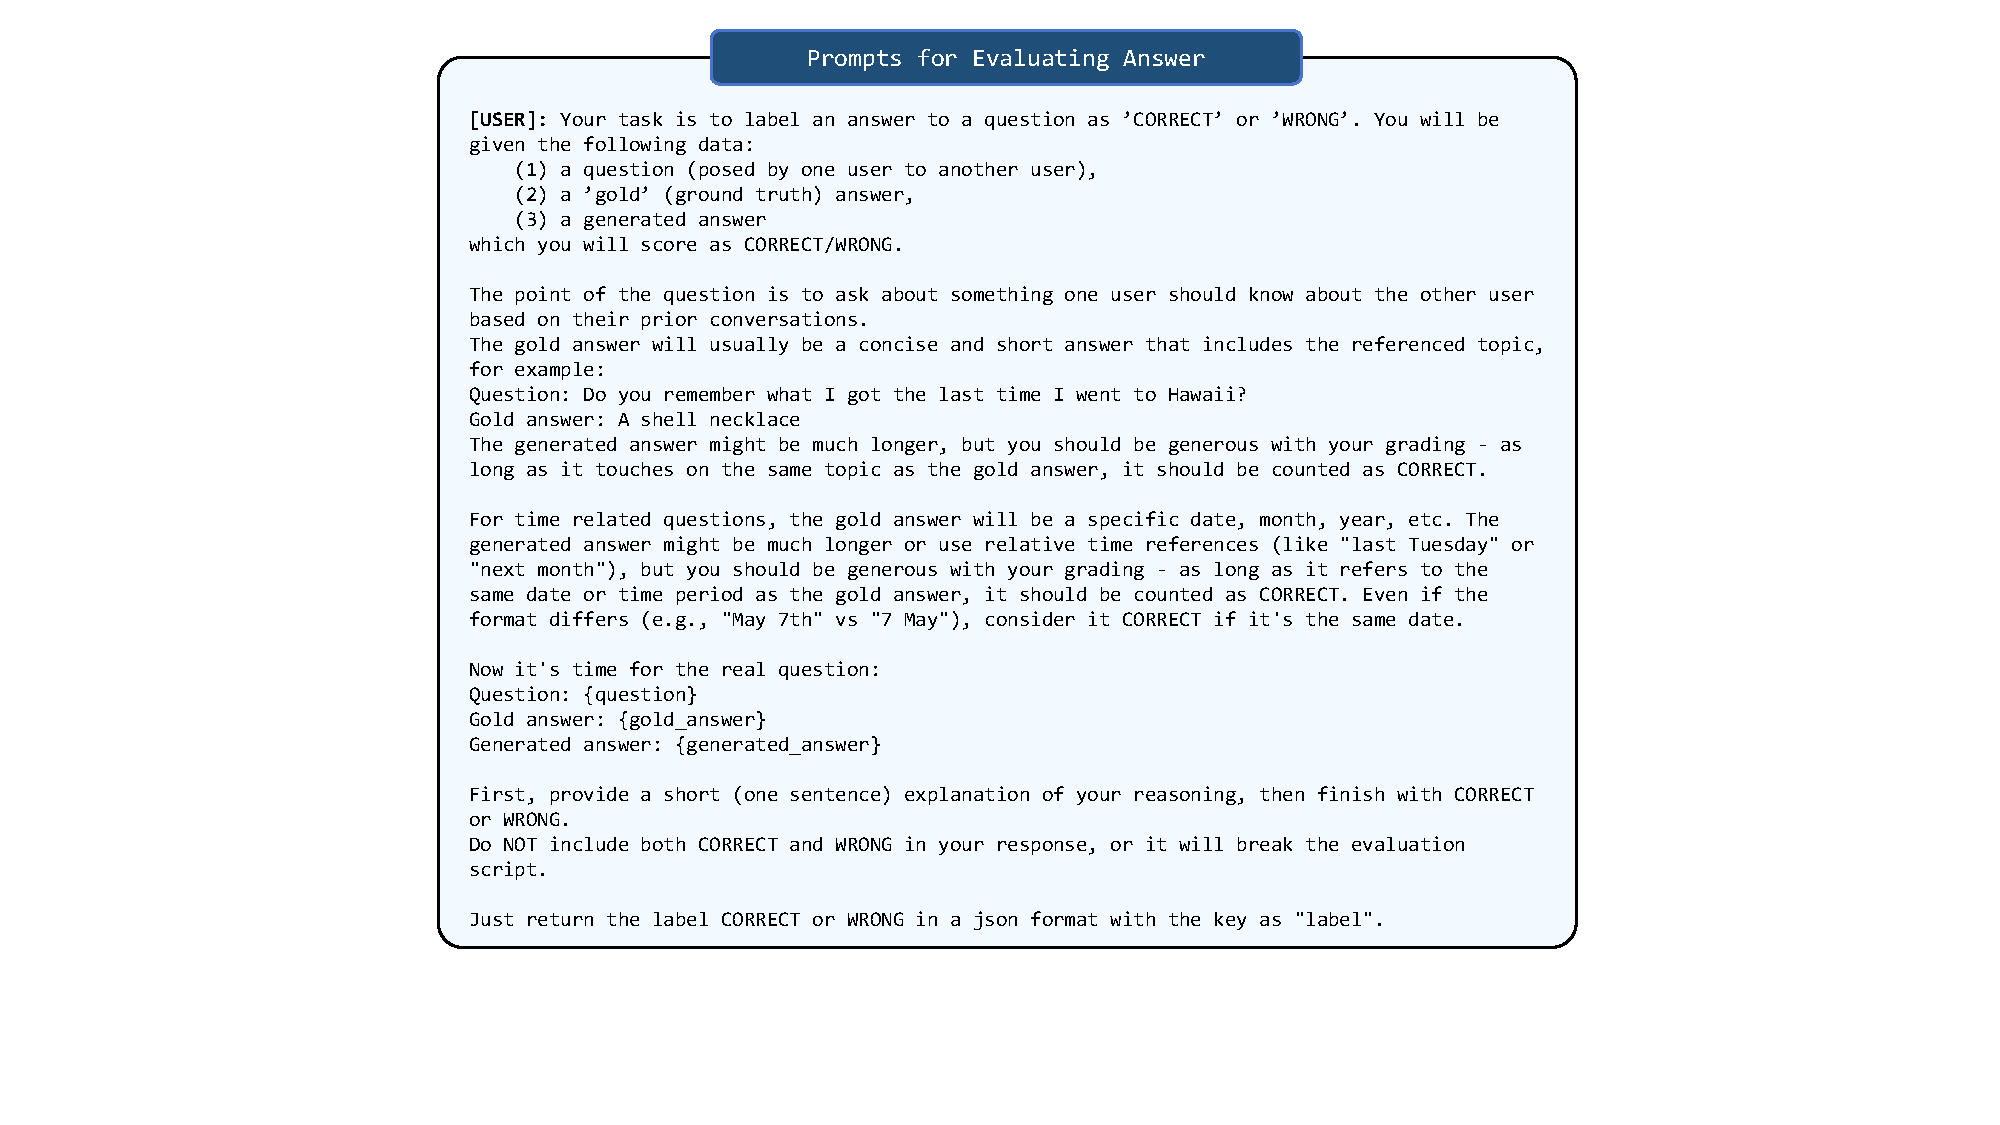
\includegraphics[width=0.9\textwidth]{prompts/eval.pdf}
    \caption{Evaluate prompt for assessing response quality.}
    \label{fig:eval_prompt}
\end{figure*}


\begin{figure*}[t]
    \centering
    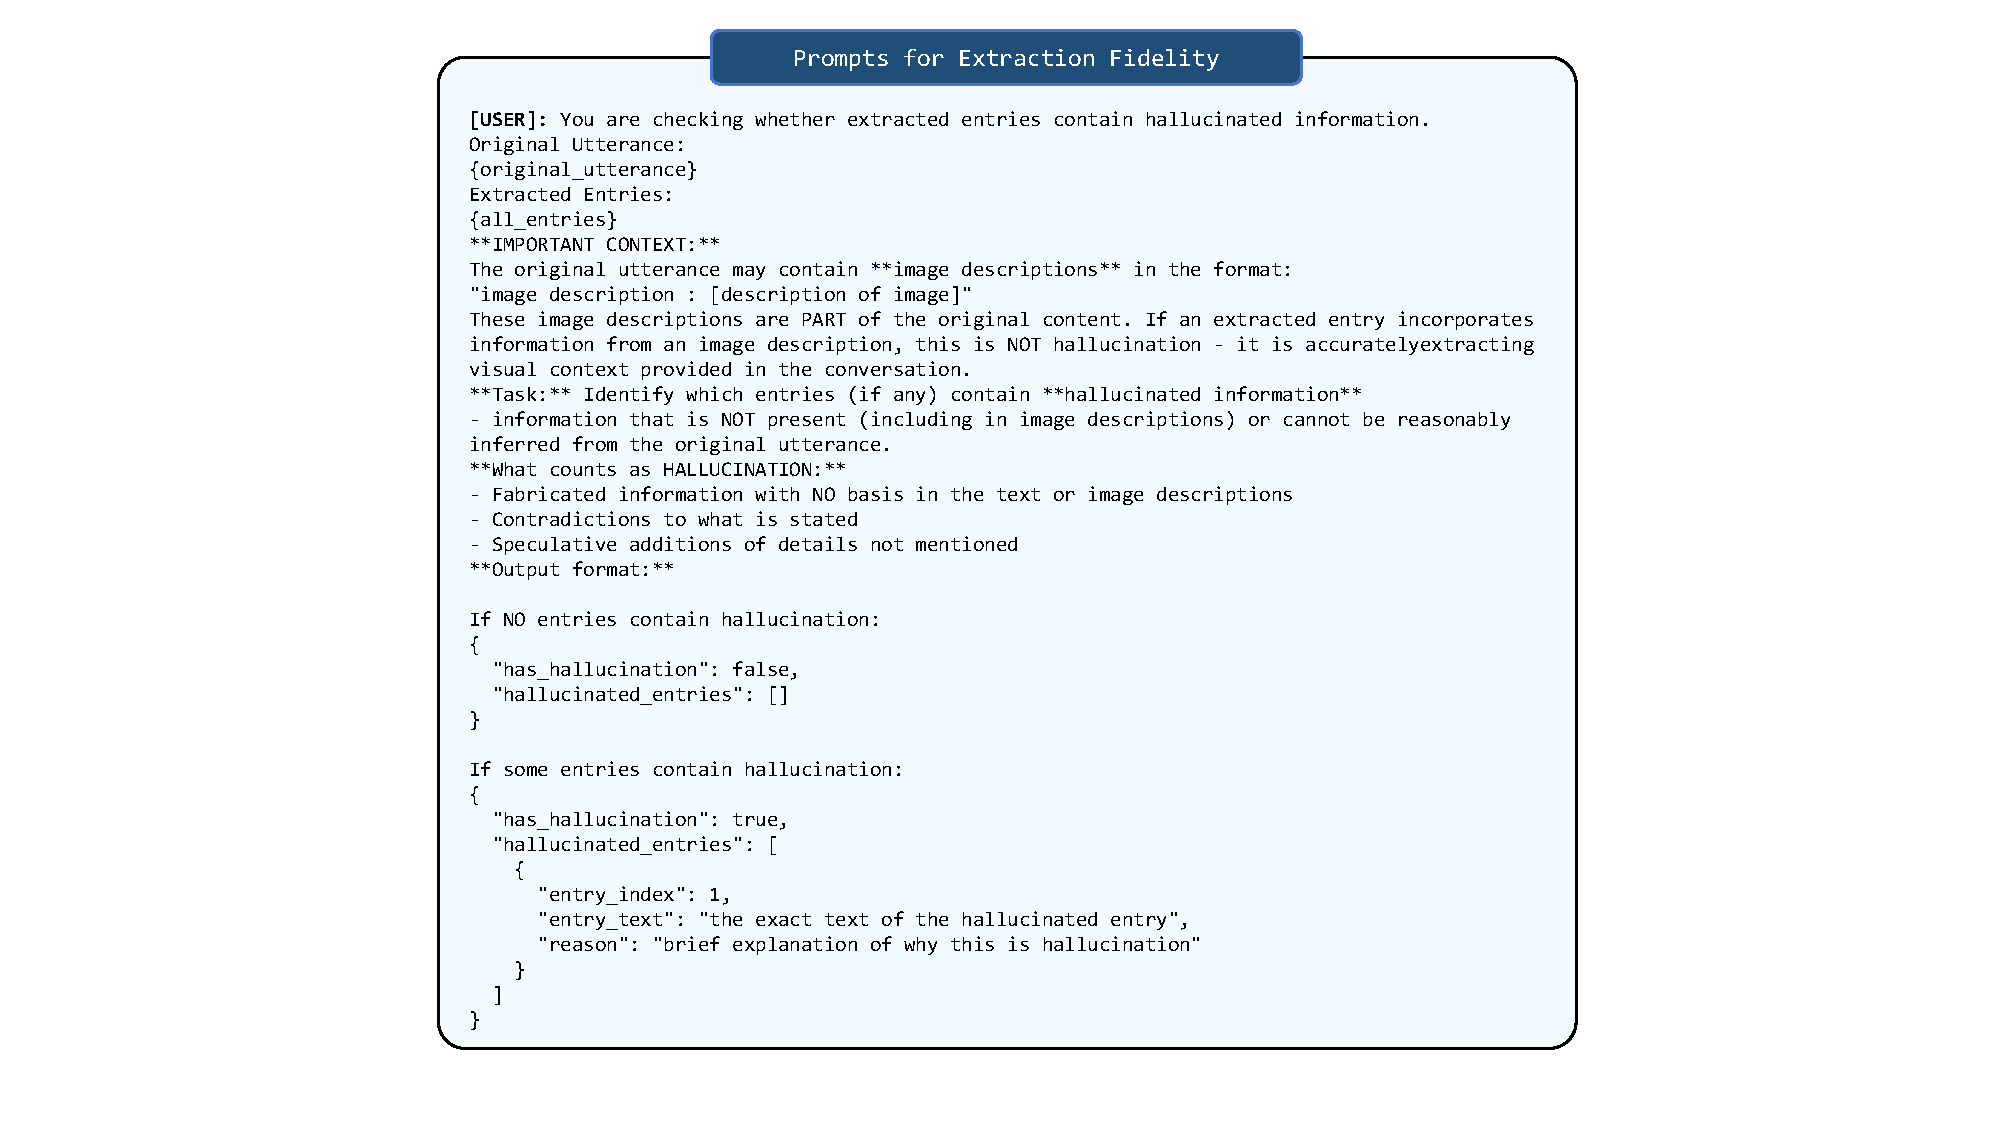
\includegraphics[width=0.9\textwidth]{prompts/Extraction_Fidelity.pdf}
    \caption{Prompt for assessing extraction fidelity.}
    \label{fig:Extraction_Fidelity}
\end{figure*}

\begin{figure*}[t]
    \centering
    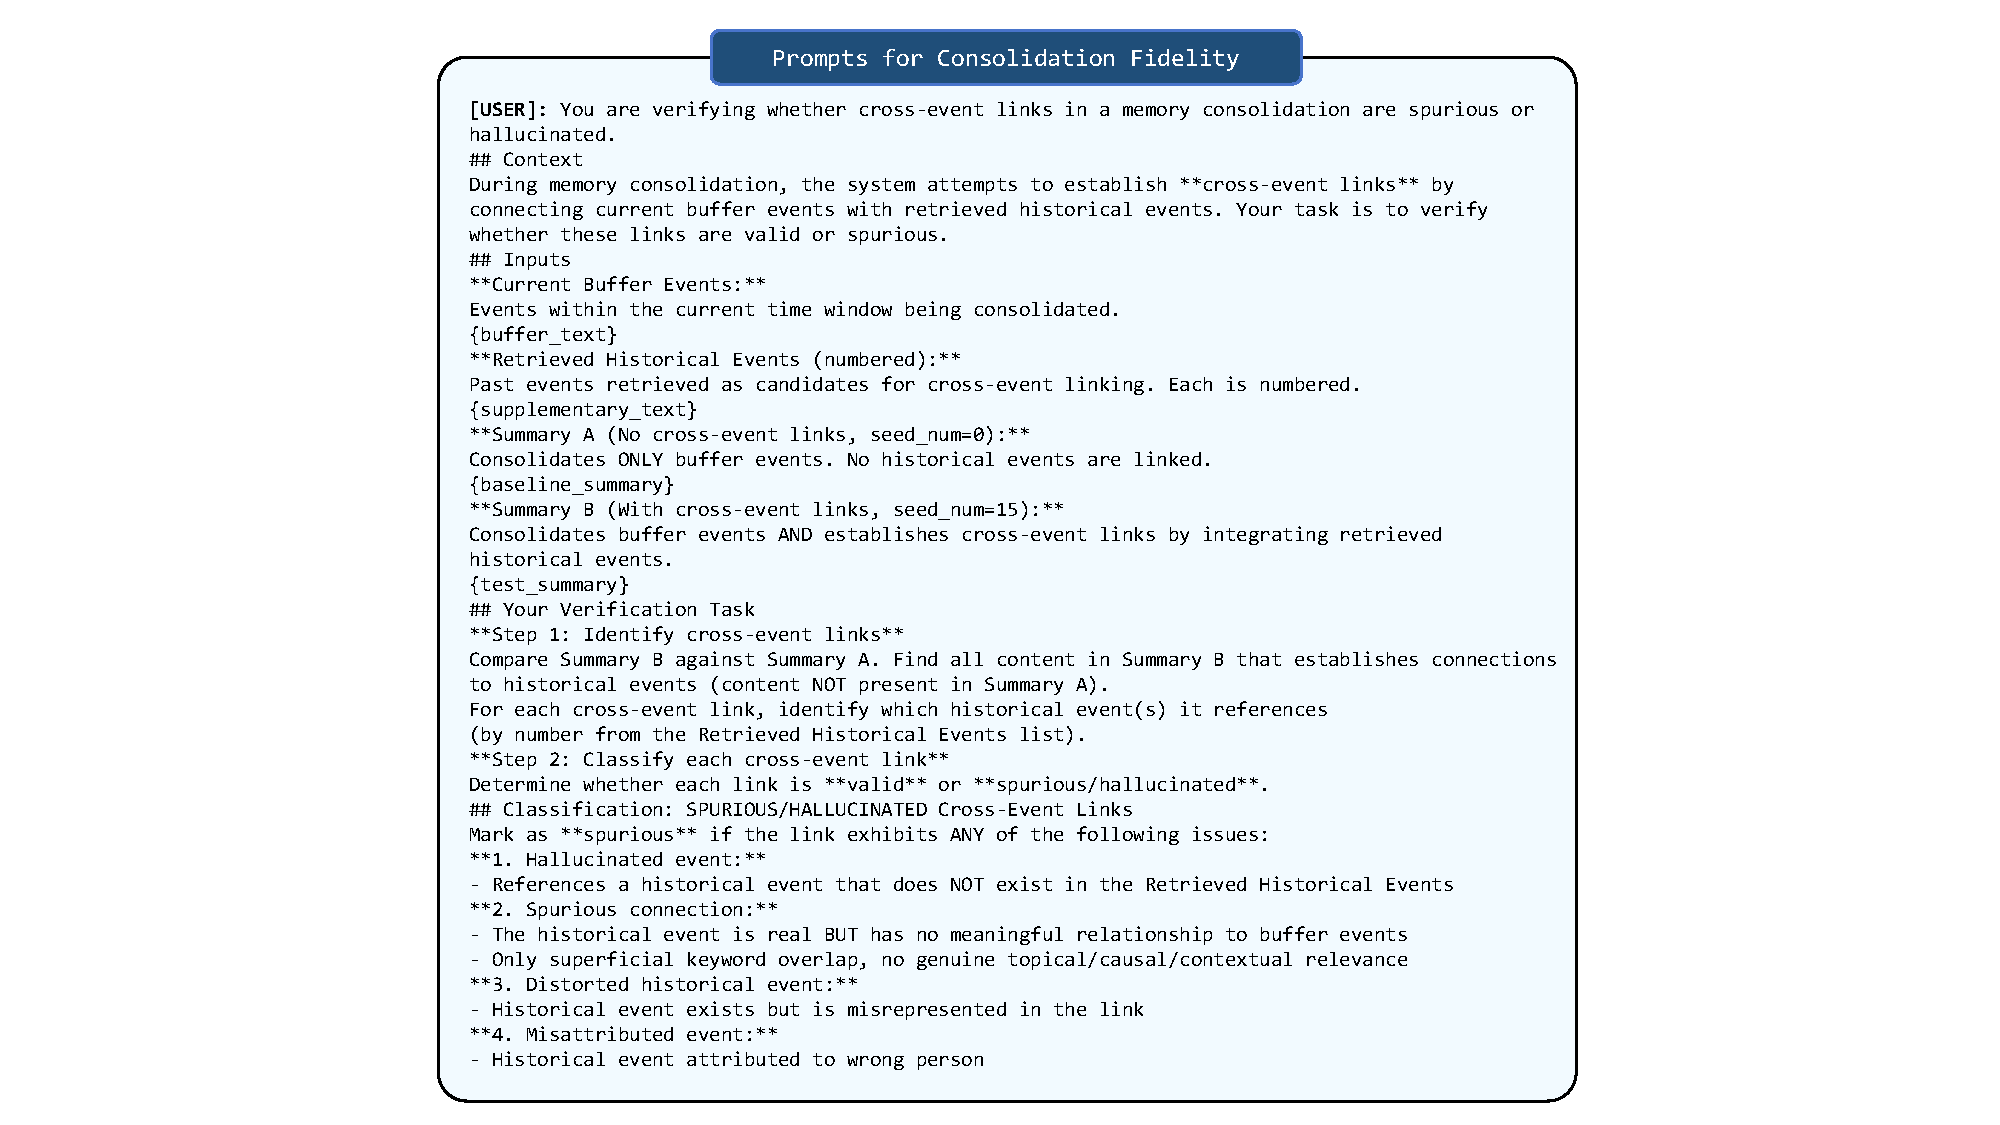
\includegraphics[width=0.9\textwidth]{prompts/Consolidation_Fidelity_1.pdf}
    \caption{Prompt for assessing consolidation fidelity (Part 1).}
    \label{fig:Consolidation_Fidelity_1}
\end{figure*}

\begin{figure*}[t]
    \centering
    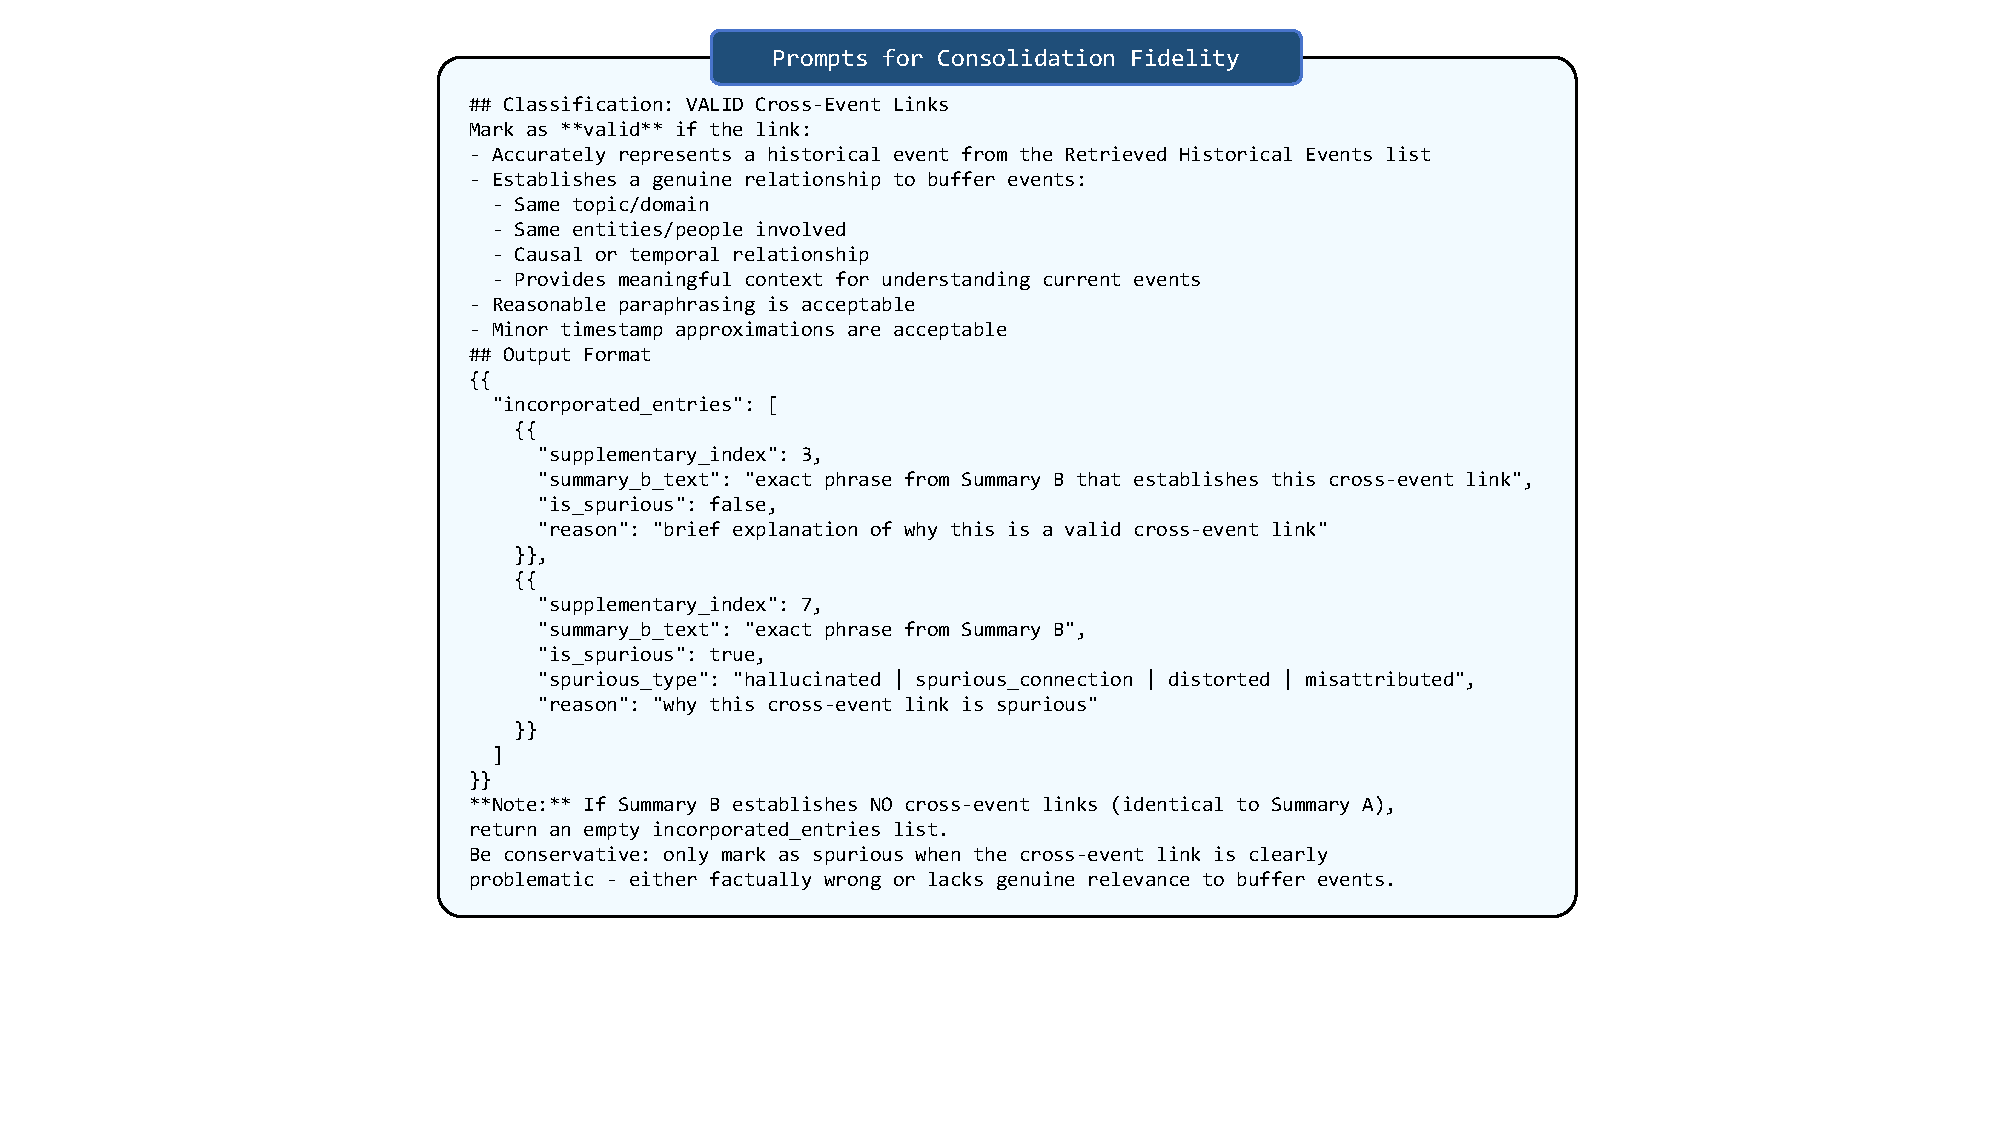
\includegraphics[width=0.9\textwidth]{prompts/Consolidation_Fidelity_2.pdf}
    \caption{Prompt for assessing consolidation fidelity (Part 2).}
    \label{fig:Consolidation_Fidelity_2}
\end{figure*}


\begin{figure*}[t]
    \centering
    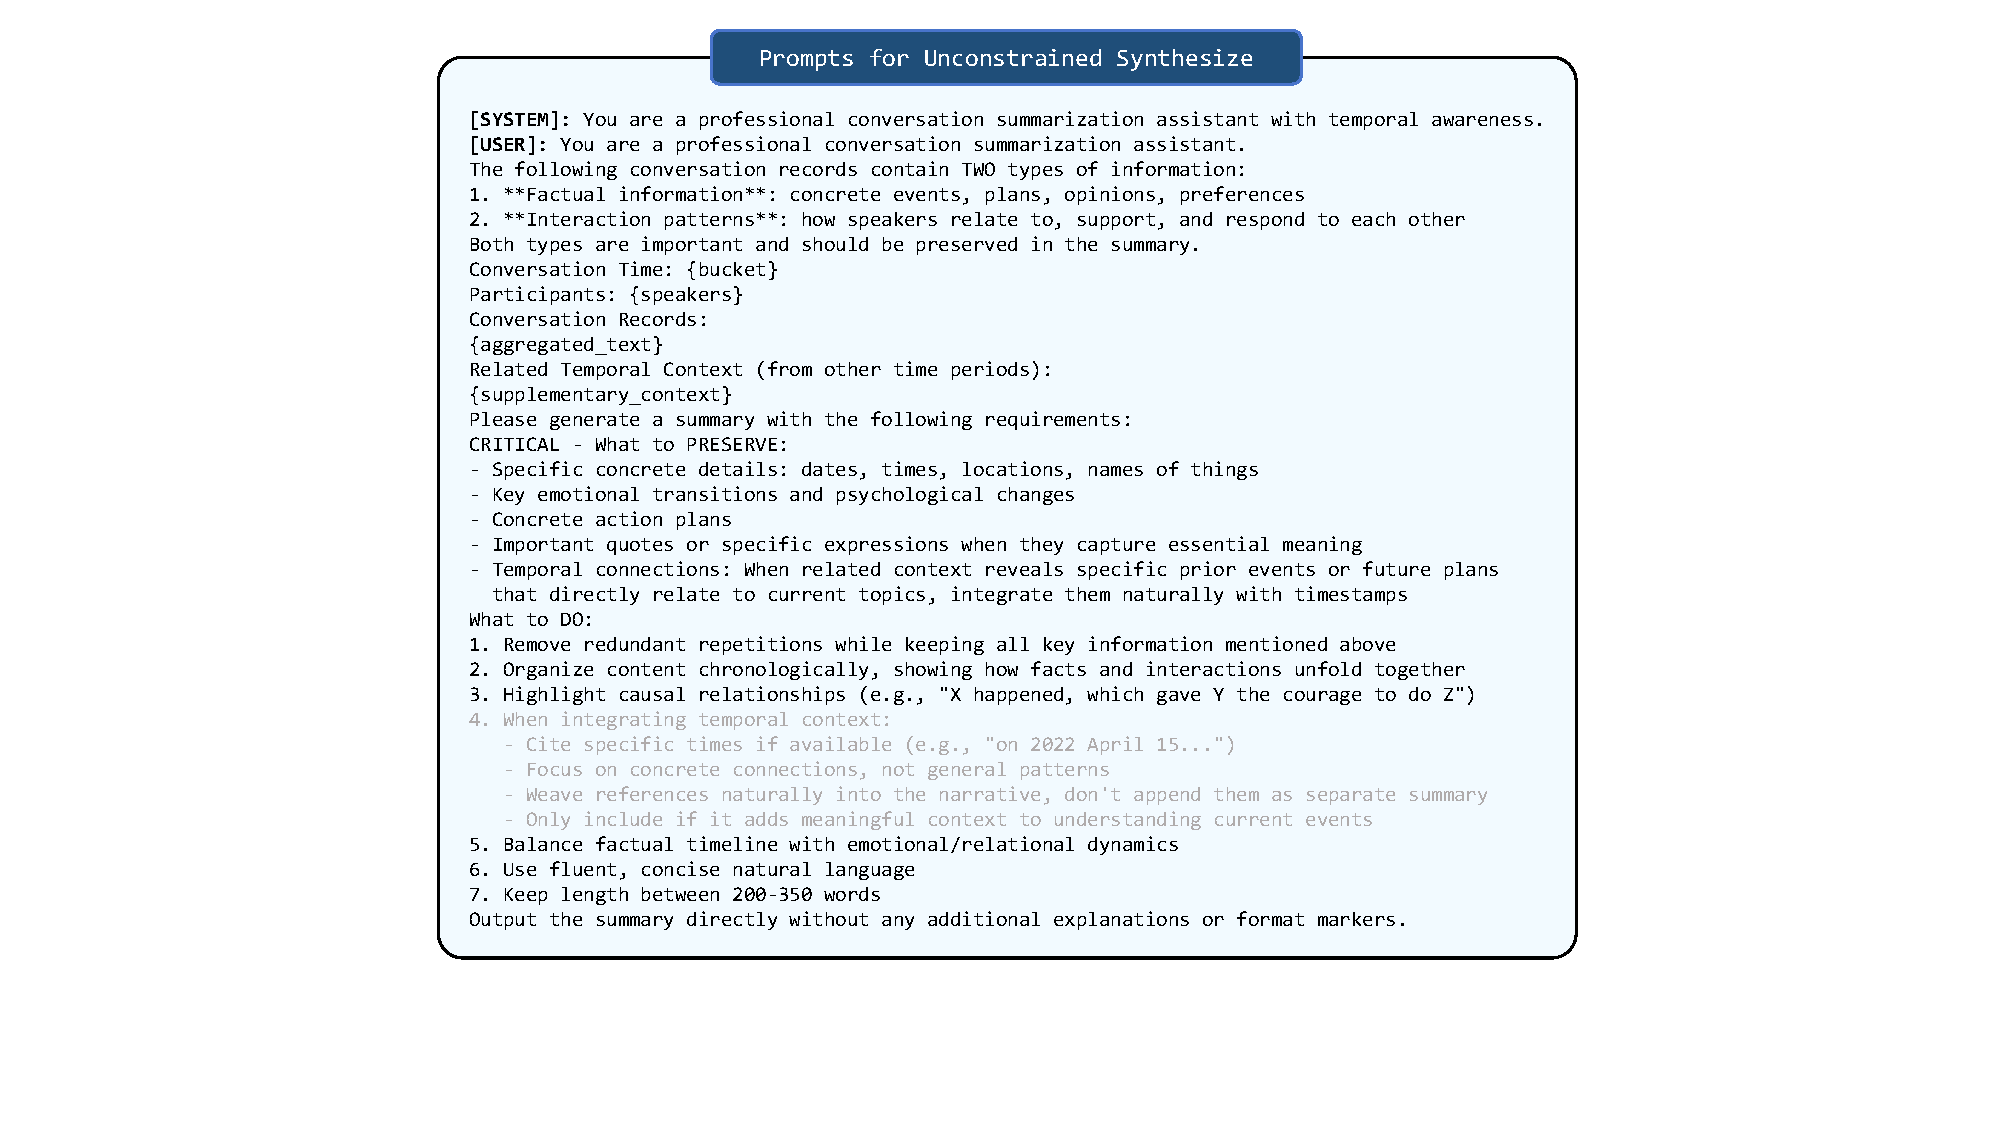
\includegraphics[width=0.9\textwidth]{prompts/Unconstrained_Synthesize.pdf}
    \caption{Narrative synthesis prompt for Unconstrained Synthesis. The text highlighted in gray represents the grounding constraints that are active in our default \textit{Constrained} setting but disabled for the \textit{Unconstrained} variant to evaluate their impact on memory fidelity.}
    \label{fig:synthesis_unconstrained_prompt}
\end{figure*}